\documentclass[11pt,a4paper]{article} % Prepara un documento con un font grande

\usepackage{iftex}

\ifLuaTeX
  % Adatta LaTeX alle convenzioni tipografiche italiane,
% e ridefinisce alcuni titoli in italiano, come "Capitolo" al posto di "Chapter",
% se il documento è in italiano
%\usepackage[italian]{babel}
%\usepackage[utf8]{inputenc} % Consente l'uso caratteri accentati italiani
%\usepackage{graphicx}		% Per le immagini
%\usepackage{gnuplot-lua-tikz}
%\usepackage[top=2.5cm, bottom=2cm, left=2cm, right=2cm]{geometry}

%\nonstopmode %non fermarti agli errori

%\usepackage{fancyhdr}
%\setlength{\headheight}{15.2pt}
%\pagestyle{fancy} % Solo le pagine normali, non i titoli nè la pagina iniziale


%%%%%%%%%%%%%%%%%%%%%%%%%%%%%%%%%%%%%%%%%%%%%%%%%%%%%%%%%%%%%%%%%%%%%%%%%%%%%%%%%%%%%%%%%

\usepackage{lipsum} % Package to generate dummy text throughout this template

\usepackage{fontspec}
\setmainfont[Ligatures=TeX]{Alegreya}

%\usepackage[sc]{mathpazo} % Use the Palatino font
%\usepackage[T1]{fontenc} % Use 8-bit encoding that has 256 glyphs
%%%%%
%\usepackage{Alegreya} %% Option 'black' gives heavier bold face 
%\renewcommand*\oldstylenums[1]{{\AlegreyaOsF #1}}

%\usepackage[euler-digits,euler-hat-accent]{eulervm}
%%%%%%
%\usepackage[utf8]{inputenc} % Consente l'uso caratteri accentati italiani
%\linespread{1.05} % Line spacing - Palatino needs more space between lines
\usepackage{amsmath, amsthm, amssymb, amsfonts}
\usepackage{microtype} % Slightly tweak font spacing for aesthetics

%%%%%%%%%%%%%%%%%%%%%%%%%%%%%%%%%%%%%%%%%%%%%
%Miei package
\usepackage[italian]{babel}
\usepackage{graphicx}		% Per le immagini
\usepackage{gnuplot-lua-tikz}
%%%%%%%%%%%%%%%%%%%%%%%%%%%%%%%%%%%%%%%%%%%%%
\usepackage[hmarginratio=1:1,top=32mm,columnsep=20pt]{geometry} % Document margins
\usepackage{multicol} % Used for the two-column layout of the document
\usepackage[hang, small,labelfont=bf,up,textfont=it,up]{caption} % Custom captions under/above floats in tables or figures
\usepackage{booktabs} % Horizontal rules in tables
\usepackage{float} % Required for tables and figures in the multi-column environment - they need to be placed in specific locations with the [H] (e.g. \begin{table}[H])
\usepackage{hyperref} % For hyperlinks in the PDF

\usepackage{lettrine} % The lettrine is the first enlarged letter at the beginning of the text
\usepackage{paralist} % Used for the compactitem environment which makes bullet points with less space between them

\usepackage{abstract} % Allows abstract customization
\renewcommand{\abstractnamefont}{\normalfont\bfseries} % Set the "Abstract" text to bold
\renewcommand{\abstracttextfont}{\normalfont\small\itshape} % Set the abstract itself to small italic text

\usepackage{titlesec} % Allows customization of titles
\renewcommand\thesection{\Roman{section}} % Roman numerals for the sections
\renewcommand\thesubsection{\Roman{subsection}} % Roman numerals for subsections
\titleformat{\section}[block]{\large\scshape\centering}{\thesection.}{1em}{} % Change the look of the section titles
\titleformat{\subsection}[block]{\large}{\thesubsection.}{1em}{} % Change the look of the section titles

\usepackage{fancyhdr} % Headers and footers
\pagestyle{fancy} % All pages have headers and footers
\fancyhead{} % Blank out the default header
\fancyfoot{} % Blank out the default footer
\fancyhead[C]{Running title $\bullet$ November 2012 $\bullet$ Vol. XXI, No. 1} % Custom header text
\fancyfoot[RO,LE]{\thepage} % Custom footer text


\else
  % Adatta LaTeX alle convenzioni tipografiche italiane,
% e ridefinisce alcuni titoli in italiano, come "Capitolo" al posto di "Chapter",
% se il documento è in italiano
%\usepackage[italian]{babel}
%\usepackage[utf8]{inputenc} % Consente l'uso caratteri accentati italiani
%\usepackage{graphicx}		% Per le immagini
%\usepackage{gnuplot-lua-tikz}
%\usepackage[top=2.5cm, bottom=2cm, left=2cm, right=2cm]{geometry}

%\nonstopmode %non fermarti agli errori

%\usepackage{fancyhdr}
%\setlength{\headheight}{15.2pt}
%\pagestyle{fancy} % Solo le pagine normali, non i titoli nè la pagina iniziale

%\usepackage{fixltx2e}
%%%%%%%%%%%%%%%%%%%%%%%%%%%%%%%%%%%%%%%%%%%%%%%%%%%%%%%%%%%%%%%%%%%%%%%%%%%%%%%%%%%%%%%%%

\usepackage{lipsum} % Package to generate dummy text throughout this template

%\usepackage[sc]{mathpazo} % Use the Palatino font
\usepackage{tgpagella} % TeX Gyre Pagella, versione migliorata di Palatino. Si ma bo, no
%\usepackage{inconsolata} % Font monospace
\usepackage{textcomp}
\usepackage[scale=0.98,ttdefault]{AnonymousPro}

%%%%%
%\usepackage{Alegreya} %% Option 'black' gives heavier bold face 
\usepackage{AlegreyaSans} %% Option 'black' gives heavier bold face 
%\renewcommand*\oldstylenums[1]{{\AlegreyaOsF #1}}
%\usepackage{opensans}
%\usepackage[euler-digits,euler-hat-accent]{eulervm}
\usepackage[euler-hat-accent]{eulervm}
%%%%%%

\usepackage[T1]{fontenc} % Use 8-bit encoding that has 256 glyphs

\usepackage[utf8]{inputenc} % Consente l'uso caratteri accentati italiani
\linespread{1.08} % Line spacing - Palatino needs more space between lines, messo a 1.08 da 1.11 che era per alegreya
\usepackage{amsmath, amsthm, amssymb, amsfonts}
\usepackage[italian]{babel}
%\usepackage[kerning,spacing,tracking,letterspace = 2,babel]{microtype} % Slightly tweak font spacing for aesthetics. Il tre è pensato per Alegreya
\usepackage[kerning,spacing,babel]{microtype}
\SetTracking[]{encoding = *,shape = *}{3} % Aumenta la distanza fra le lettere
							     % http://tex.stackexchange.com/questions/66494/new-command-for-spacing-letters-in-microtype
%%%%%%%%%%%%%%%%%%%%%%%%%%%%%%%%%%%%%%%%%%%%%
%Miei package



\usepackage{graphicx}		% Per le immagini
%\usepackage{color}		% COLORI!

%\definecolor{grigio-molto-scuro}{gray}{0.1}	%colore

\usepackage{tabularx}		% Per le tabelle con le colonne tutte uguali
\usepackage{tabulary}		% Tabelle migliorate, nelle celle il testo va a capo da solo...
\usepackage{gnuplot-lua-tikz}
%%%%%%%%%%%%%%%%%%%%%%%%%%%%%%%%%%%%%%%%%%%%%
\newlength{\alphabet}
\settowidth{\alphabet}{\normalfont abcdefghijklmnopqrstuvwxyz}
\usepackage[
	    %hmargin=0.18\paperwidth,% metti la larghezza del testo (margini orizzontali) al 18% del foglio
	    textwidth=2.5\alphabet,  % http://tex.stackexchange.com/questions/59626/nicely-force-66-characters-per-line
	    hmarginratio=1:1,       % margini destro e sinistro uguali
	    top=35mm,	            % margine sopra a 32mm...
	    vmarginratio=4:5,       % quello sotto uguale (default 2:3)
	    columnsep=20pt]         % Spazio tra le colonne?
	    {geometry} % Document margins
\usepackage{multicol} % Used for the two-column layout of the document
\usepackage[hang, small,labelfont=bf,up,textfont=it,up]{caption} % Custom captions under/above floats in tables or figures
\usepackage{booktabs} % Horizontal rules in tables
\usepackage{float} % Required for tables and figures in the multi-column environment - they need to be placed in specific locations with the [H] (e.g. \begin{table}[H])
%\usepackage{tocloft} % Per customizzare le liste di floats (per i custom float!)
\usepackage[titles]{tocloft} %Pare causi meno casini con fancyhdr
\usepackage{nicefrac} % Per le frazioni tipo ⅛
\usepackage{pdfpages} % Per includere pagine intere in pdf (per la copertina)
%\usepackage[squaren]{siunitx}

\usepackage{lettrine} % The lettrine is the first enlarged letter at the beginning of the text
\usepackage{paralist} % Used for the compactitem environment which makes bullet points with less space between them
\usepackage[section]{placeins} % Per \FloatBarrier. L'opzione section comporta che le sezioni siano floatbarriers

\usepackage{abstract} % Allows abstract customization
\renewcommand{\abstractnamefont}{\normalfont\bfseries} % Set the "Abstract" text to bold
\renewcommand{\abstracttextfont}{\normalfont\small\itshape} % Set the abstract itself to small italic text

\usepackage{caption} % Per captions avanzate

\usepackage{listingsutf8} % Per includere codice sorgente meglio che con verbatim (e con caratteri non inglesi)
\lstset{ 
  %Preso anche questo da http://en.wikibooks.org/wiki/LaTeX/Source_Code_Listings
  %backgroundcolor=\color{white},   % choose the background color; you must add \usepackage{color} or \usepackage{xcolor}
  basicstyle=\footnotesize\ttfamily,        % the size of the fonts that are used for the code E MESSO IN MONOSPACE
  breakatwhitespace=true,         % sets if automatic breaks should only happen at whitespace
  breaklines=true,                 % sets automatic line breaking
  captionpos=b,                    % sets the caption-position to bottom
  %commentstyle=\color{mygreen},    % comment style
  %deletekeywords={...},            % if you want to delete keywords from the given language
  %escapeinside={\%*}{*)},          % if you want to add LaTeX within your code
  %extendedchars=true,              % lets you use non-ASCII characters; for 8-bits encodings only, does not work with UTF-8
  frame=l,                    % adds a frame around the code
				    %you can control the rules at the top, right, bottom, and left directly by using the four initial 
				    %letters for single rules and their upper case versions for double rules. http://mirror.hmc.edu/ctan/macros/latex/contrib/listings/listings.pdf
				    % Es frame frame=trBL ha doppia linea a sinistra e sotto, e singola a destra e sopra
  keepspaces=true,                 % keeps spaces in text, useful for keeping indentation of code (possibly needs columns=flexible)
  %keywordstyle=\color{blue},       % keyword style
  %language=Octave,                 % the language of the code
  %morekeywords={*,...},            % if you want to add more keywords to the set
  numbers=left,                    % where to put the line-numbers; possible values are (none, left, right)
  numbersep=5pt,                   % how far the line-numbers are from the code
  %numberstyle=\tiny\color{mygray}, % the style that is used for the line-numbers
  %rulecolor=\color{black},         % if not set, the frame-color may be changed on line-breaks within not-black text (e.g. comments (green here))
  showspaces=false,                % show spaces everywhere adding particular underscores; it overrides 'showstringspaces'
  showstringspaces=false,          % underline spaces within strings only
  showtabs=false,                  % show tabs within strings adding particular underscores
  stepnumber=1,                    % the step between two line-numbers. If it's 1, each line will be numbered
  %stringstyle=\color{mymauve},     % string literal style
  tabsize=2,                       % sets default tabsize to 2 spaces
  title=\lstname                   % show the filename of files included with \lstinputlisting; also try caption instead of title
}


\usepackage{titlesec} % Allows customization of titles
\renewcommand\thesection{\Roman{section}} % Roman numerals for the sections
\renewcommand\thesubsection{\Roman{subsection}} % Roman numerals for subsections
% \usefont {encoding} {family} {series} {shape}
\titleformat{\section}[block]{\AlegreyaSansSC \bfseries \LARGE}{\thesection.}{1em}{} % Change the look of the section titles. Pezzi spostati \scshape\centering\bfseries
\titleformat{\subsection}[block]{\AlegreyaSans \bfseries \Large}{\thesection.\thesubsection }{1em}{} % Change the look of the section titles

\usepackage{fancyhdr} % Headers and footers
\pagestyle{fancy} % All pages have headers and footers
\fancyhead{} % Blank out the default header
\fancyfoot{} % Blank out the default footer
\headheight=14pt % Perchè sennò continua a lamentarsi che 12pt è troppo poco e la mette a 14 lo stesso
%\fancyhead[C]{Chiappara, Labanca, Forcher - \textit{Ottica geometrica} $\bullet$ \thesection}
\fancyhead[L]{\textit{Relazione di Spettroscopia}} % Custom header text. \nouppercase{\leftmark} per sezione, ma non ci sta
\fancyhead[R]{\textsc{\nouppercase{\leftmark}}}
\fancyfoot[RO,LE]{\thepage} % Custom footer text

\usepackage[hidelinks]{hyperref} % For hyperlinks in the PDF
\hypersetup{
    bookmarks=true,         % show bookmarks bar?
    unicode=false,          % non-Latin characters in Acrobat’s bookmarks
   % pdftoolbar=true,        % show Acrobat’s toolbar?
   % pdfmenubar=true,        % show Acrobat’s menu?
   % pdffitwindow=false,     % window fit to page when opened
    %pdfstartview={FitH},    % fits the width of the page to the window
    pdftitle={Relazione di Spettroscopia},    % title
    pdfauthor={L. Buonincontri, E. Lusiani, F. Forcher},     % author
    pdfsubject={Relazione di Spettroscopia - Laboratorio 2016},   % subject of the document
    %pdfcreator={Creator},   % creator of the document
    %pdfproducer={Producer}, % producer of the document
    pdfkeywords={spettroscopia} {relazione} {Sperimentazioni}, % list of keywords
    %pdfnewwindow=true,      % links in new PDF window
    %colorlinks=false,       % false: boxed links; true: colored links
    linkcolor=red,          % color of internal links (change box color with linkbordercolor)
    citecolor=green,        % color of links to bibliography
    filecolor=magenta,      % color of file links
    urlcolor=cyan           % color of external links
}

\fi
\DeclareGraphicsExtensions{.pdf, .png, .jpg} % Se due immagini hanno lo stesso nome sceglile secondo l'ordine di filetype qui
\graphicspath{ {./img/} }					 % Path delle immagini 

\title{
\vspace{-3cm}
\fontsize{48pt}{10pt}\selectfont
\textsc{Relazione di \\[3mm] Spettroscopia} \\[8mm] 
\fontsize{24pt}{10pt}\selectfont
\textit{Camera di Bragg}
}
% \title{}
\author{
\large
\textsc{Francesco Forcher}\\[2mm]
\normalsize Università di Padova, Facoltà di Fisica\\
\normalsize \texttt{francesco.forcher@studenti.unipd.it}\\
\normalsize Matricola: \texttt{1073458}\\
\and
\large
\textsc{Enrico Lusiani}\\[2mm]
\normalsize Università di Padova, Facoltà di Fisica\\
\normalsize \texttt{enrico.lusiani@studenti.unipd.it}\\
\normalsize Matricola: \texttt{1073300}\\
\and
\large
\textsc{Laura Buonincontri}\\[2mm]
\normalsize Università di Padova, Facoltà di Fisica\\
\normalsize \texttt{laura.buonincontri@studenti.unipd.it}\\
\normalsize Matricola: \texttt{1073131}
}
\date{\today}

%%%%%%%%%%%%%%%%%%%%%%%%%%%%%%%%%%%%%%5%%%%%%%%%%%%%%%%%%%%%%%%%%%%%%%%%%%%%%%%%%%
%\usepackage{float}
%\usepackage{caption}
%\usepackage{multirow}
%\usepackage[top=3.6cm, bottom=1.5in, left=0.5in, right=0.5in]{geometry}

%%%%%%%%%%%%%%%%%
% Robe del package tocloft per fare gli indici delle mie tabelle e grafici
% texblog.org/2008/07/13/define-your-own-list-of/
%\newcommand{\listtabellaname}{Lista delle tabelle}
%\newlistof{tabella}{tab}{\listtabellaname}


%%%%%%%%%%%%%%%%%

% I miei stili di float, con le righe
\floatstyle{plaintop}
\newfloat{tabella}{tb}{lop} 
\floatname{tabella}{Tabella}

\floatstyle{ruled}
\newfloat{grafico}{tb}{loi} 
\floatname{grafico}{Grafico}

\newcommand{\tabellaautorefname}{\bfseries Tabella} % per \autoref del package hyperref
\newcommand{\graficoautorefname}{\bfseries Grafico} % Idem



%%%%%%%%%%%%%%%%%%%%%%%%%%%%%%%%%%%%%%%%%%%%%%%%%%%%%%%%%%%%%%%%%%%%%5%%%%%%%%%%%%%
% Comandi personalizzati

% \newcommand{\cm}{\,\mathrm{cm}}
% \DeclareMathOperator{\cov}{cov} % Covarianza
% \DeclareMathOperator{\var}{var} % Covarianza
% \newcommand{\mm}{\,\mathrm{mm}}
% \newcommand{\nm}{\,\mathrm{nm}}
% \newcommand{\usuq}{\nicefrac{1}{q}}
% \newcommand{\usup}{\nicefrac{1}{p}}



%////////////////////////////////////////////////////////////////////////////////////////////////////////////////////////////
%////////////////////////////////////////////////////////////////////////////////////////////////////////////////////////////
% Fine dei dati iniziali per il latex: il documento finale inizierà da qui
\begin{document}

%\includepdf[pages={1}]{./img/copertina_relazione.pdf}

{
%\color{grigio-molto-scuro}
%\lsstyle % Abilita il letterspacing personalizzato
%\unclfamily % Cagata per il font Uncial

\maketitle % Produce il titolo a partire dai comandi \title, \author e \date

\vspace{ \stretch{1} }
\begin{center}
	%non si poteva non mettere
	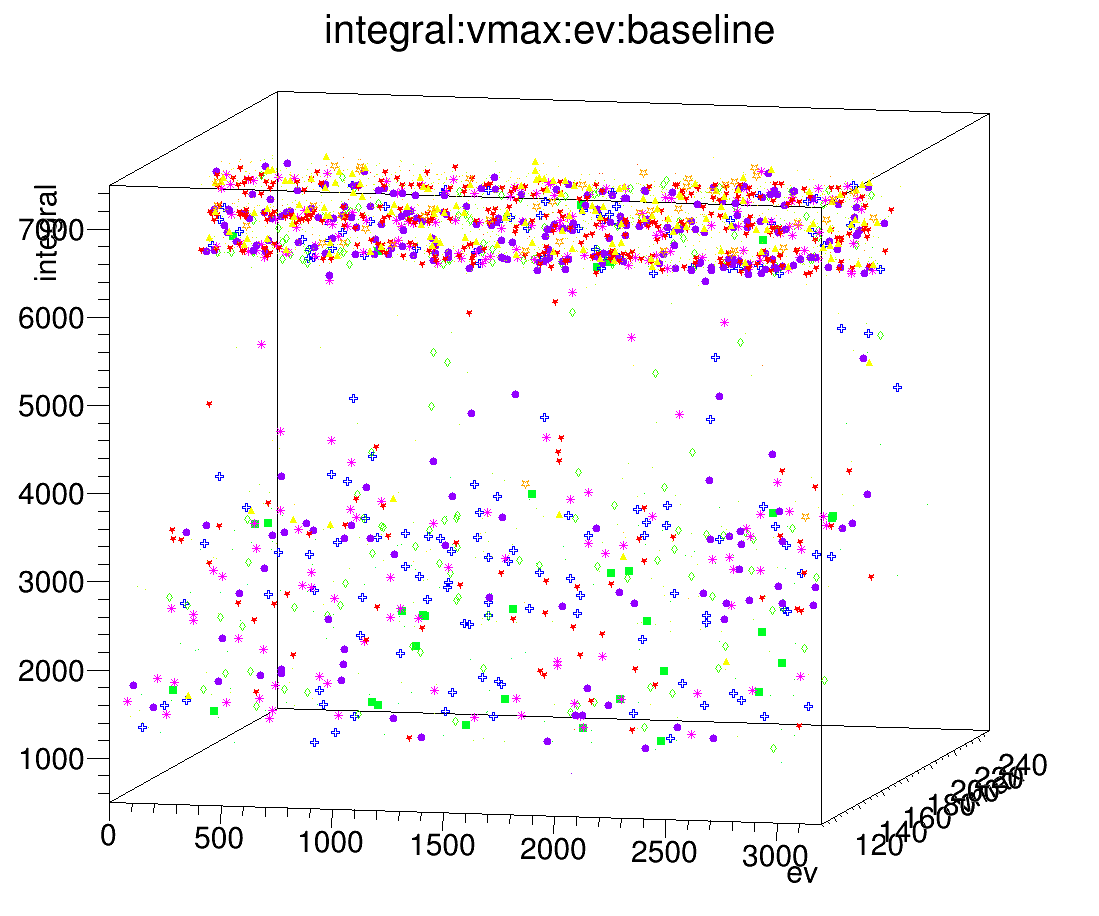
\includegraphics[width=0.7\textwidth]{stelle_di_natale_quadrimensionale.png}
	%\caption{Una NTupla in 4D} 
\end{center}

%\vspace{ \stretch{1} }
\newpage
% Le varie sezioni
%\section{Obiettivi}
\begin{abstract}
	\noindent
	L'obiettivo dell'esperienza è la misura della curva di trasferimento di un amplificatore (in configurazione invertente e non invertente) e 
lo studio della sua risposta in frequenza (in configurazione non invertente).

\end{abstract}

\newpage


\microtypesetup{protrusion=false} % disables protrusion locally in the document
\tableofcontents % prints Table of Contents
%\listoftabella
%\listoffigures
%\listoftables
\microtypesetup{protrusion=true} % enables protrusion

%\begin{multicols}{2}

\section{Schema camera}
	Da aggiungere, forse l'immagine che c'è anche nelle istruzioni?


% \section{Metodologia di misura}
% 	\input{./sezioni/metodologia_misura.tex}

%\newpage
%\end{multicols}
% \section{Presentazione dei dati}
 	%inserire circuito
\section{Parte I}
\subsection{Prima misura delle particelle alfa}
Sono stati settati gli strumenti, a pressione 600 $mb$.
Si è mantenuto lo Shaping Time a 0.25-0.5 $\mu s$, dopo aver osservato il comportamento. %dire cosa succede
E' stata regolata l'amplificazione in modo da mantenere il picco attorno ai $3V$.
E' stato impostato il trigger in modo tale che fosse circa a metà altezza del picco sull'oscilloscopio. 

%Avevamo visto che a 1,5 V dovevamo impostare circa 96 nel trigger in binario, ma poi, non ricordo per che motivo, abbiamo alzato a 128 tipo

Si è verificato che il numero di segnali spuri fosse inferiore al $30 \%$ del totale, facendo il grafico dei picchi e calcolando l'integrale dei segnali a bassa energia.

E' stato quindi acquisito il primo set di dati (circa 3000 eventi)

\begin{grafico}
 \centering
 \resizebox{\textwidth}{!}{%
 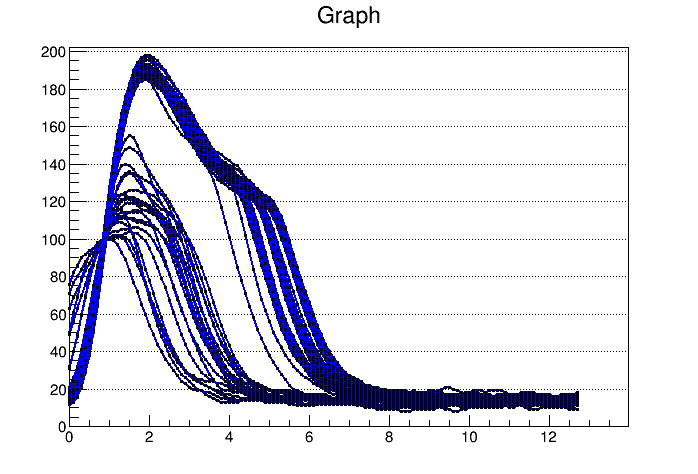
\includegraphics{../grafici/risultati/misura600.png}
 }%
 \caption{Grafico segnali a 600mb} 
 \label{gr:misura_600} 
\end{grafico}


E' stato acquisito anche un set di dati con meno eventi per stimare la baseline.
In particolare, è stato calcolato il centroide del picco della baseline, da inserire nella macro al posto del valore di default.

\begin{grafico}
 \centering
 \resizebox{\textwidth}{!}{%
 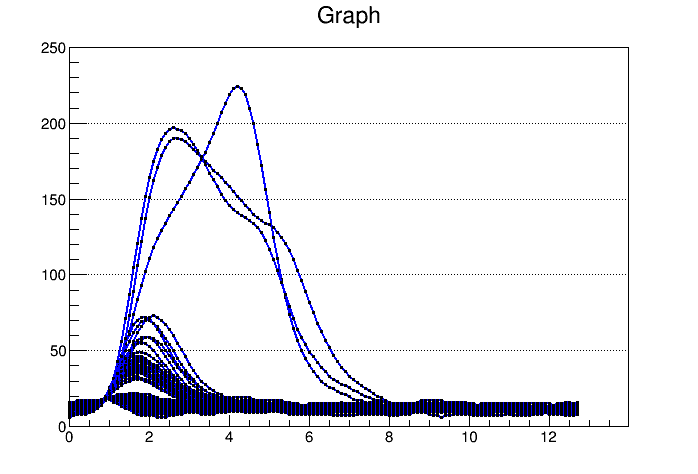
\includegraphics{../grafici/risultati/misura600fondo.png}
 }%
 \caption{Grafico segnali baseline} 
 \label{gr:misura600fondo} 
\end{grafico}

E' stato fatto il grafico degli integrali ed è stato calcolato il centroide del picco della baseline, da inserire nella macro al posto del valore di default.

\begin{grafico}
 \centering
 \resizebox{\textwidth}{!}{%
 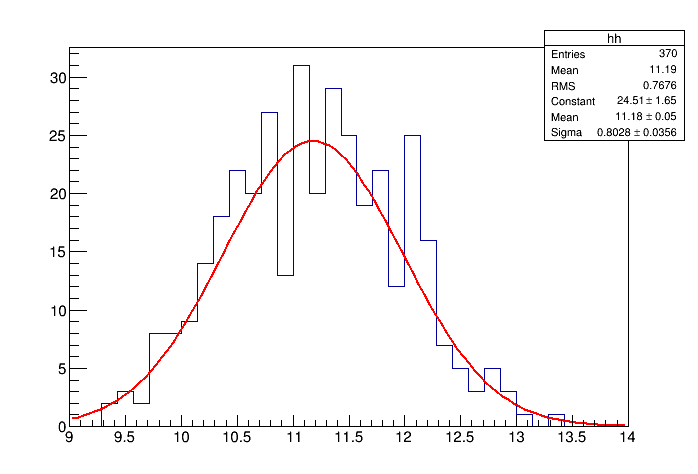
\includegraphics{../grafici/risultati/misura600fondo_baseline.png}
 }%
 \caption{Picco della baseline} 
 \label{gr:misura600fondo_baseline} 
\end{grafico}
%dati baseline

L'analisi dei dati che segue è stata effettuata utilizzando la macro fornite dal laboratorio,
modificando il limite dei campioni da integrare e inserendo il valore della baseline appena stimato.
Il limite dei campioni a 600 mb è stato posto uguale a 90.

\begin{grafico}
 \centering
 \resizebox{\textwidth}{!}{%
 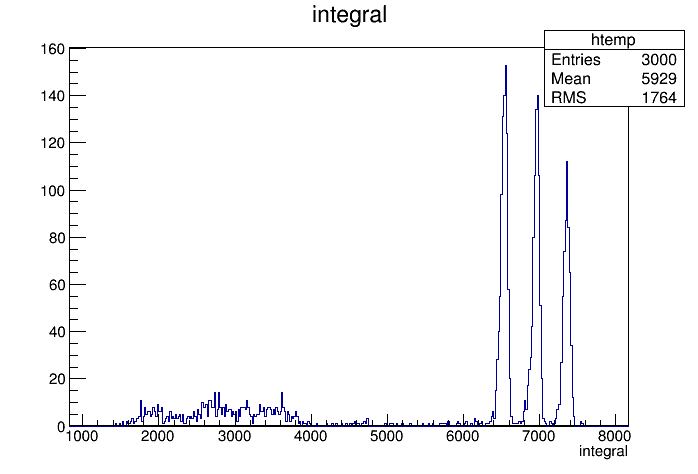
\includegraphics{../grafici/risultati/misura600_integral.png}
 }%
 \caption{Grafico integrale} 
 \label{gr:misura600_integral} 
\end{grafico}

 \begin{grafico}
 \centering
 \resizebox{\textwidth}{!}{%
 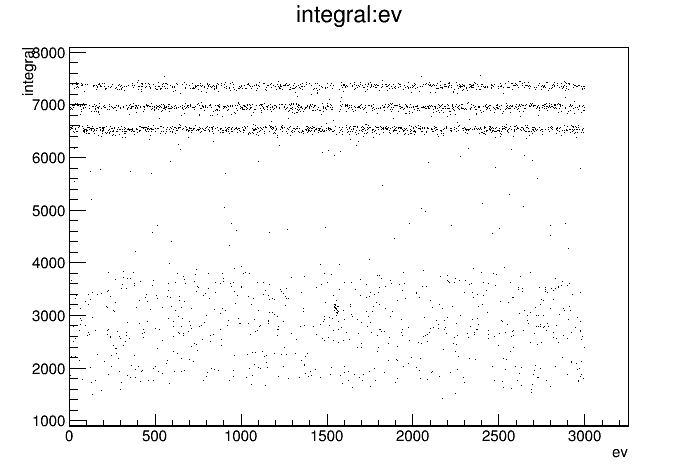
\includegraphics{../grafici/risultati/misura600_integral_ev.png}
 }%
 \caption{Grafico integral:ev} 
 \label{gr:misura600_integral_ev} 
\end{grafico}

 \begin{grafico}
 \centering
 \resizebox{\textwidth}{!}{%
 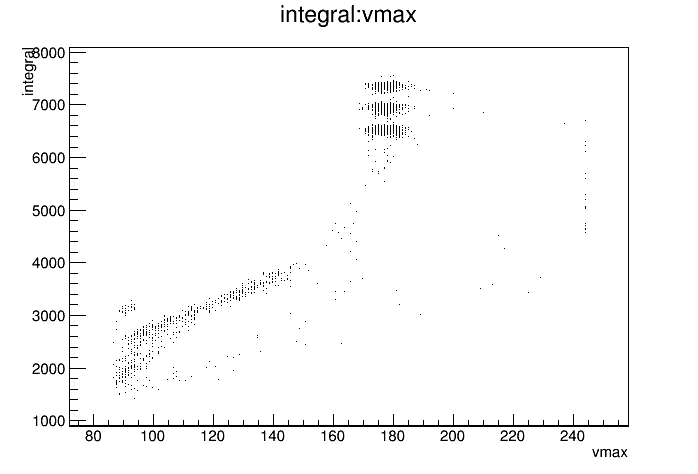
\includegraphics{../grafici/risultati/misura600_integral_vmax.png}
 }%
 \caption{Grafico integral:vmax} 
 \label{gr:misura600_integral_vmax} 
\end{grafico}

\begin{grafico}
 \centering
 \resizebox{\textwidth}{!}{%
 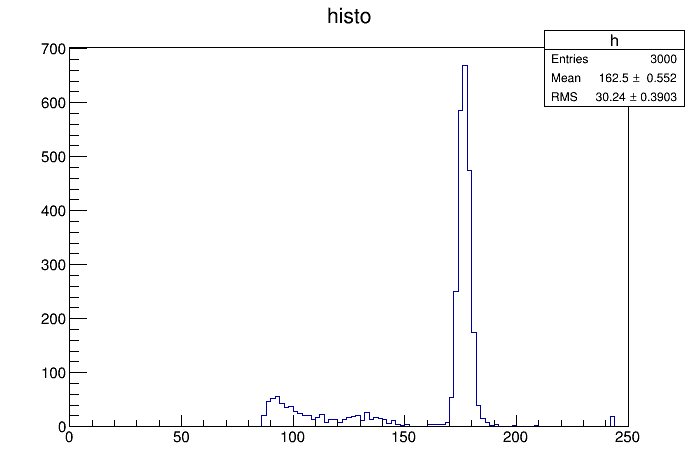
\includegraphics{../grafici/risultati/misura600_vmax.png}
 }%
 \caption{Grafico vmax} 
 \label{gr:misura600_vmax} 
\end{grafico}

 \begin{grafico}
 \centering
 \resizebox{\textwidth}{!}{%
 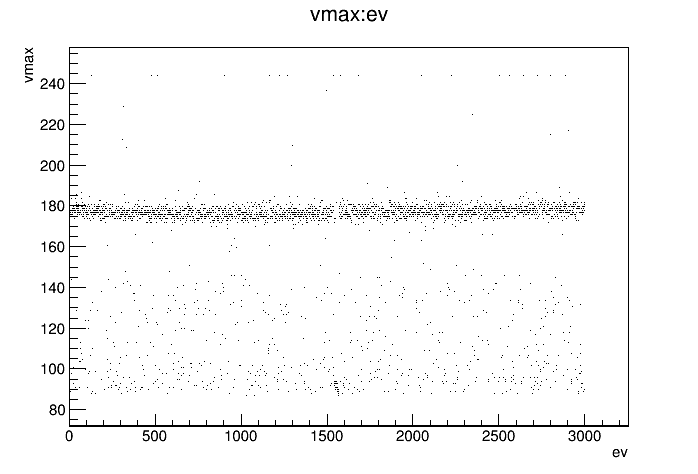
\includegraphics{../grafici/risultati/misura600_vmax_ev.png}
 }%
 \caption{Grafico vmax:ev} 
 \label{gr:misura600_vmax_ev} 
\end{grafico}

\subsection{Risoluzione energetica}
\subsection{Risoluzione energetica}
\FloatBarrier
Per il calcolo della risoluzione energetica, abbiamo per prima cosa trovata la relazione tra integrale ed energia, ipotizzandola lineare. 
Per fare ciò abbiamo calcolato l'energia teorica di ciscun picco, facendo la media delle energie dei decadimenti alfa, pesate sulla loro probabilità. 
Poi abbiamo calcolato l'integrale relativo a ciascun picco, come centroide del picco nell'istogramma degli integrali, e il suo errore, l'RMS del picco.
Da questi dati abbiamo proceduto ad un interpolazione dell'integrale in funzione dell'energia, ricavando così la funzione energia:integrale. 
Usando la funzione, abbiamo riscalato l'asse delle ascisse nell'istogramma degli integrali, in modo che mostrasse l'energia. 
Da questo nuovo istogramma abbiamo ricavato la risoluzione energetica, misurando l'RMS dei picchi e usandola per la formula

TODO fatemela bene voi la formula qui, non so fare le equazioni

$$risoluzione=\frac{2.335\cdot\sigma_E}{E}$$

\begin{grafico}
 \centering
 \resizebox{\textwidth}{!}{%
 \input{../grafici/risultati/energy_integral.tex}
 }%
 \caption{Grafico Energia:Integrale} 
 \label{gr:energy_integral.tex} 
\end{grafico}

TODO fate voi anche qui
$$q=19.6792\pm19.5559$$
$$m=1.2469\pm0.00354684$$

\begin{grafico}
 \centering
 \resizebox{\textwidth}{!}{%
 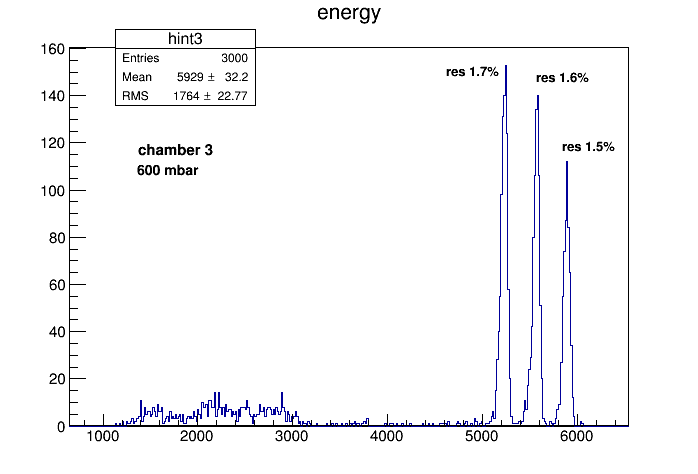
\includegraphics{../grafici/risultati/misura600_energy.png}
 }%
 \caption{Risoluzioni energetiche, grafico Energia(keV):conteggio} 
 \label{gr:600_energy.tex} 
\end{grafico}

\FloatBarrier

\FloatBarrier

\section{Parte II}
\section{Parte II}
L'analisi dei dati che segue è stata effettuata utilizzando la macro fornite dal laboratorio,
modificando il limite dei campioni e inserendo il valore della baseline stimato in precedenza.

\subsection{Misure a pressione 650mb}
\FloatBarrier

\begin{grafico}[H]
 \centering
 \resizebox{\textwidth}{!}{%
 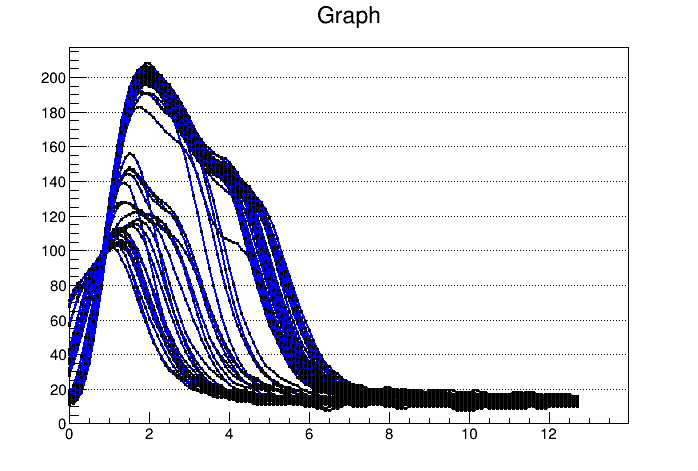
\includegraphics{../grafici/risultati/misura650.png}
 }%
 \caption{Grafico segnali a 650mb}
 \label{gr:misura_650} 
\end{grafico}

\begin{grafico}[H]
 \centering
 \resizebox{\textwidth}{!}{%
 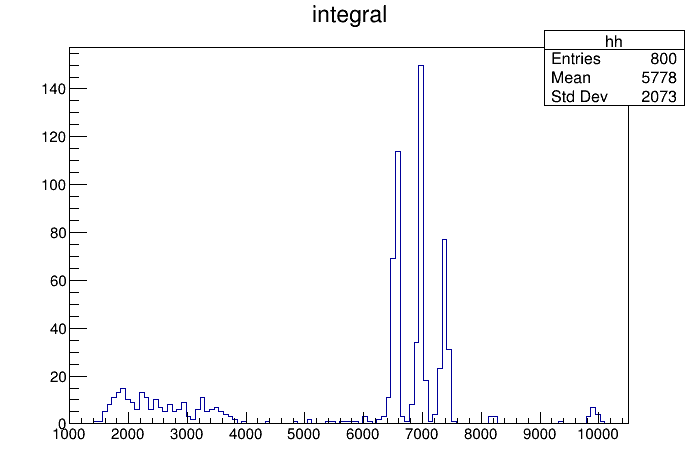
\includegraphics{../grafici/risultati/misura650_integral.png}
 }%
 \caption{Grafico integrale} 
 \label{gr:misura650_integral} 
\end{grafico}

 \begin{grafico}
 \centering
 \resizebox{\textwidth}{!}{%
 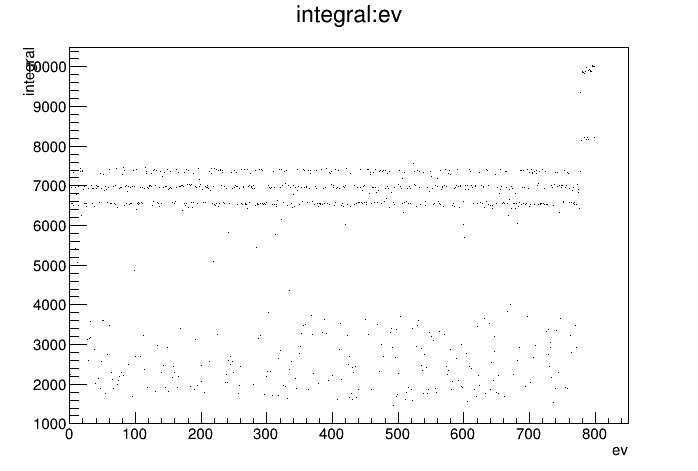
\includegraphics{../grafici/risultati/misura650_integral_ev.png}
 }%
 \caption{Grafico integral:ev} 
 \label{gr:misura650_integral_ev} 
\end{grafico}

 \begin{grafico}
 \centering
 \resizebox{\textwidth}{!}{%
 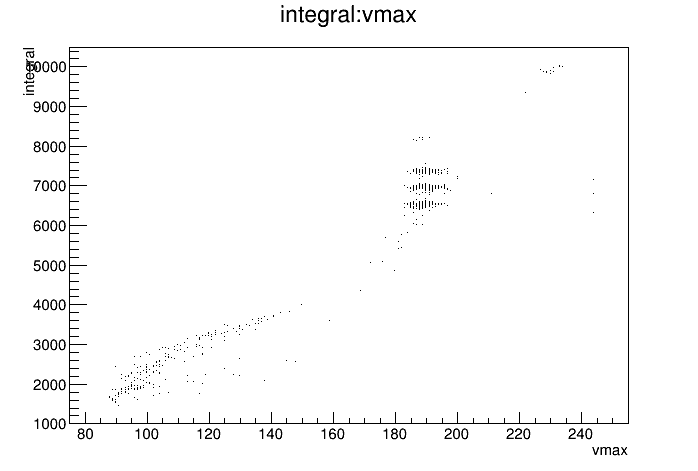
\includegraphics{../grafici/risultati/misura650_integral_vmax.png}
 }%
 \caption{Grafico integral:vmax} 
 \label{gr:misura650_integral_vmax} 
\end{grafico}

\begin{grafico}
 \centering
 \resizebox{\textwidth}{!}{%
 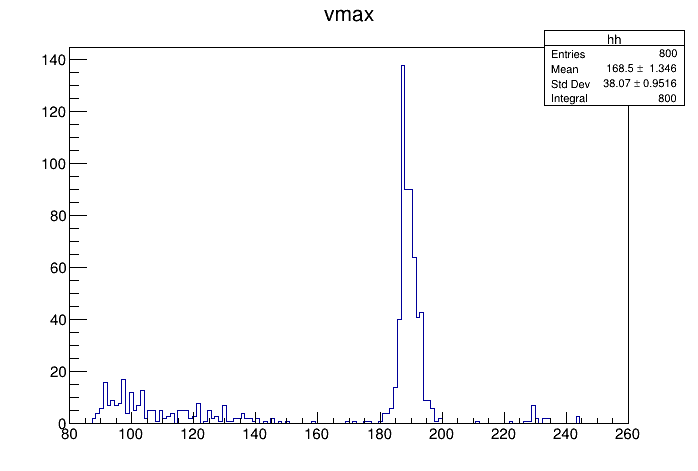
\includegraphics{../grafici/risultati/misura650_vmax.png}
 }%
 \caption{Grafico vmax} 
 \label{gr:misura650_vmax} 
\end{grafico}

 \begin{grafico}
 \centering
 \resizebox{\textwidth}{!}{%
 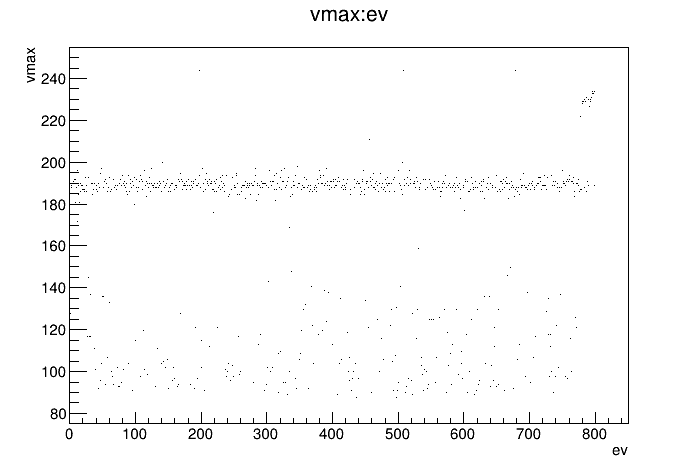
\includegraphics{../grafici/risultati/misura650_vmax_ev.png}
 }%
 \caption{Grafico vmax:ev} 
 \label{gr:misura650_vmax_ev} 
\end{grafico}

\FloatBarrier

\subsection{Misure a pressione 550mb}
\FloatBarrier

\begin{grafico}
 \centering
 \resizebox{\textwidth}{!}{%
 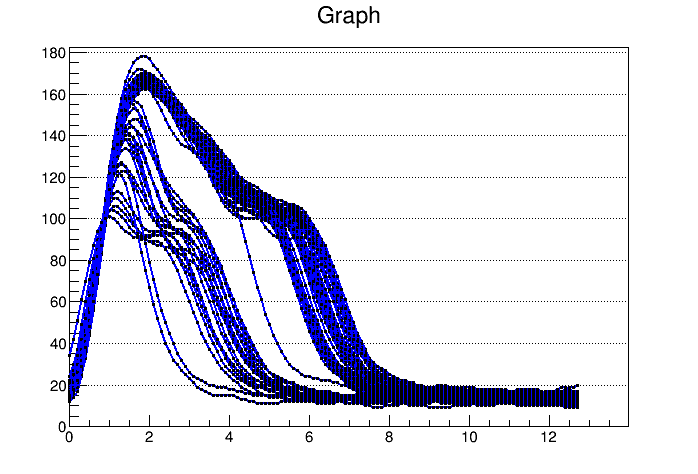
\includegraphics{../grafici/risultati/misura550.png}
 }%
 \caption{Grafico segnali a 550mb} 
 \label{gr:misura_550} 
\end{grafico}

\begin{grafico}
 \centering
 \resizebox{\textwidth}{!}{%
 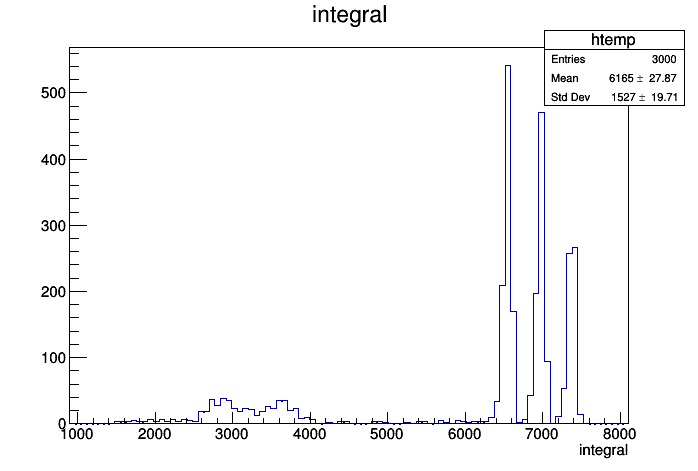
\includegraphics{../grafici/risultati/misura550_integral.png}
 }%
 \caption{Grafico integrale} 
 \label{gr:misura550_integral} 
\end{grafico}

 \begin{grafico}
 \centering
 \resizebox{\textwidth}{!}{%
 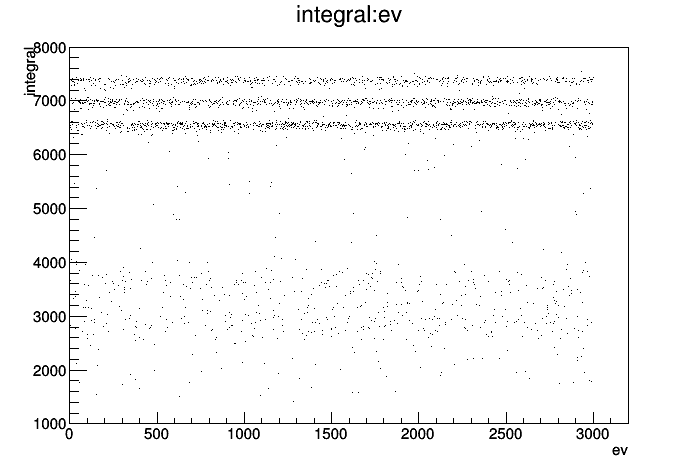
\includegraphics{../grafici/risultati/misura550_integral_ev.png}
 }%
 \caption{Grafico integral:ev} 
 \label{gr:misura550_integral_ev} 
\end{grafico}

 \begin{grafico}
 \centering
 \resizebox{\textwidth}{!}{%
 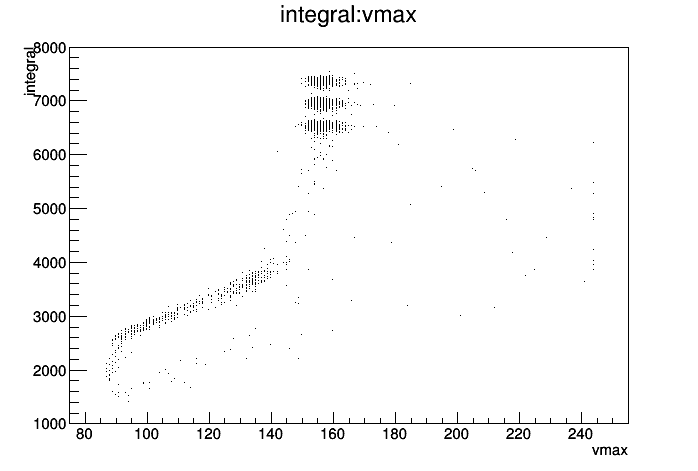
\includegraphics{../grafici/risultati/misura550_integral_vmax.png}
 }%
 \caption{Grafico integral:vmax} 
 \label{gr:misura550_integral_vmax} 
\end{grafico}

\begin{grafico}
 \centering
 \resizebox{\textwidth}{!}{%
 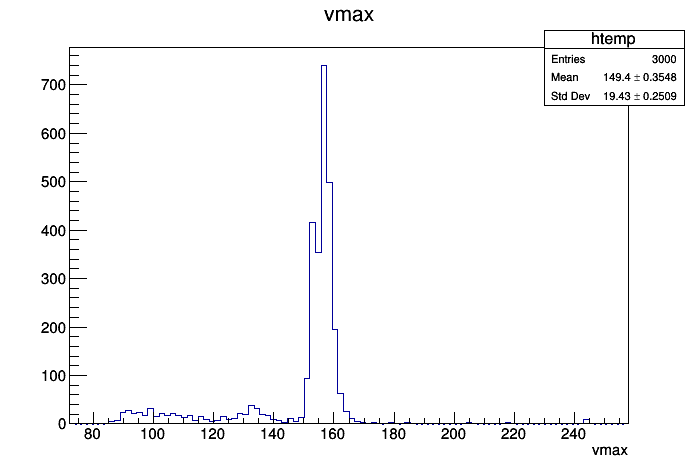
\includegraphics{../grafici/risultati/misura550_vmax.png}
 }%
 \caption{Grafico vmax} 
 \label{gr:misura550_vmax} 
\end{grafico}

 \begin{grafico}
 \centering
 \resizebox{\textwidth}{!}{%
 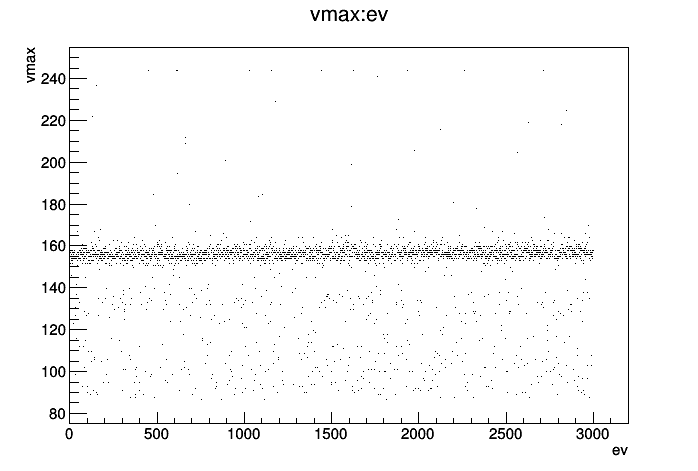
\includegraphics{../grafici/risultati/misura550_vmax_ev.png}
 }%
 \caption{Grafico vmax:ev} 
 \label{gr:misura550_vmax_ev} 
\end{grafico}

\FloatBarrier

\subsection{Misure a pressione 500mb}
\FloatBarrier

\begin{grafico}
 \centering
 \resizebox{\textwidth}{!}{%
 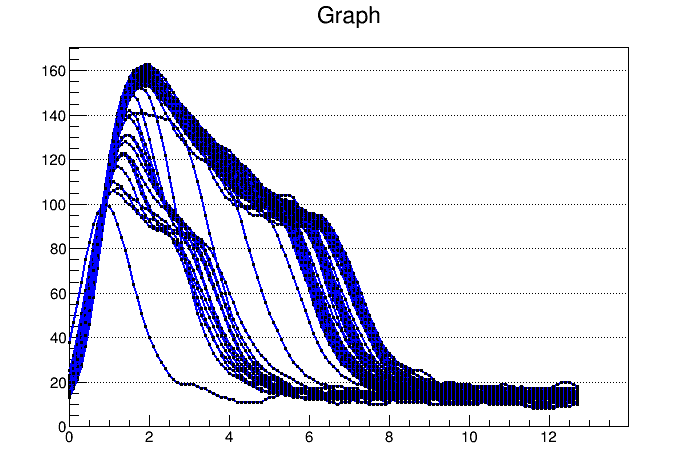
\includegraphics{../grafici/risultati/misura500.png}
 }%
 \caption{Grafico segnali a 500mb} 
 \label{gr:misura_500} 
\end{grafico}

\begin{grafico}
 \centering
 \resizebox{\textwidth}{!}{%
 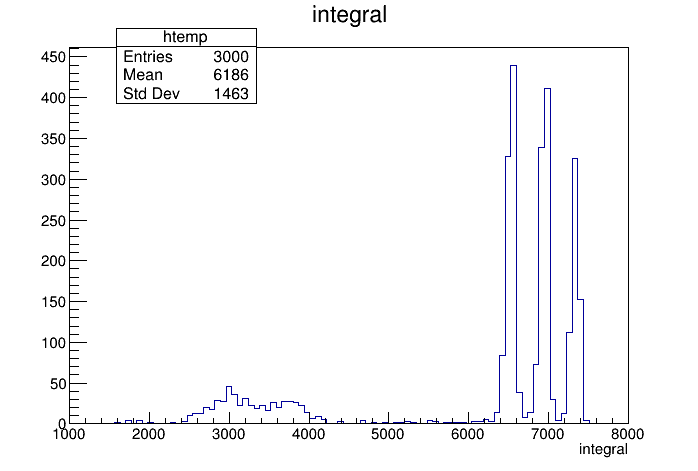
\includegraphics{../grafici/risultati/misura500_integral.png}
 }%
 \caption{Grafico integrale} 
 \label{gr:misura500_integral} 
\end{grafico}

 \begin{grafico}
 \centering
 \resizebox{\textwidth}{!}{%
 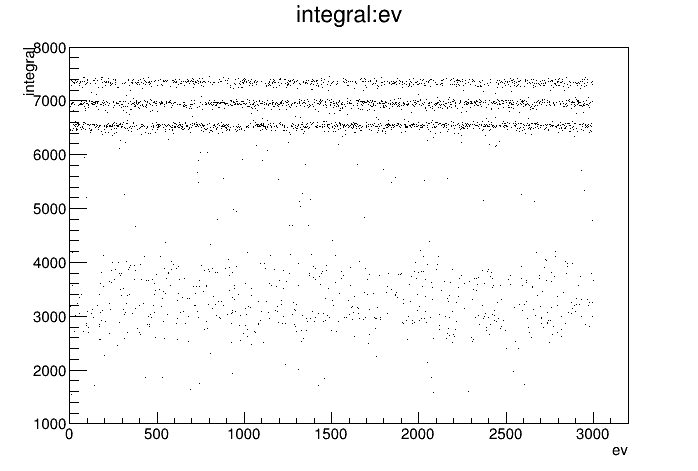
\includegraphics{../grafici/risultati/misura500_integral_ev.png}
 }%
 \caption{Grafico integral:ev} 
 \label{gr:misura500_integral_ev} 
\end{grafico}

 \begin{grafico}
 \centering
 \resizebox{\textwidth}{!}{%
 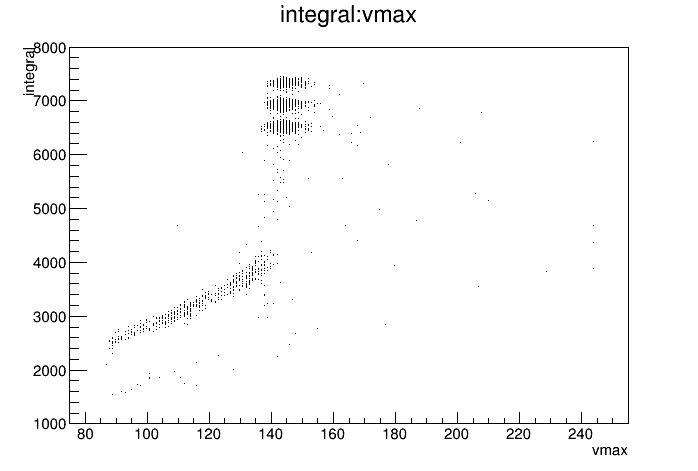
\includegraphics{../grafici/risultati/misura500_integral_vmax.png}
 }%
 \caption{Grafico integral:vmax} 
 \label{gr:misura500_integral_vmax} 
\end{grafico}

\begin{grafico}
 \centering
 \resizebox{\textwidth}{!}{%
 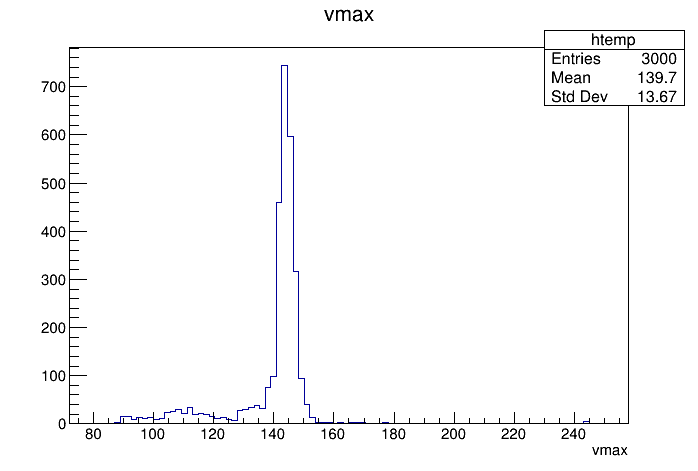
\includegraphics{../grafici/risultati/misura500_vmax.png}
 }%
 \caption{Grafico vmax} 
 \label{gr:misura500_vmax} 
\end{grafico}

 \begin{grafico}
 \centering
 \resizebox{\textwidth}{!}{%
 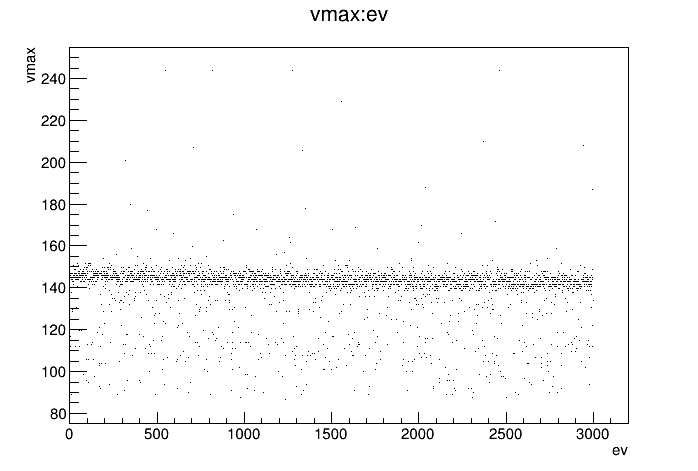
\includegraphics{../grafici/risultati/misura500_vmax_ev.png}
 }%
 \caption{Grafico vmax:ev} 
 \label{gr:misura500_vmax_ev} 
\end{grafico}

\FloatBarrier

\subsection{Misure a pressione 450mb}
\FloatBarrier

\begin{grafico}
 \centering
 \resizebox{\textwidth}{!}{%
 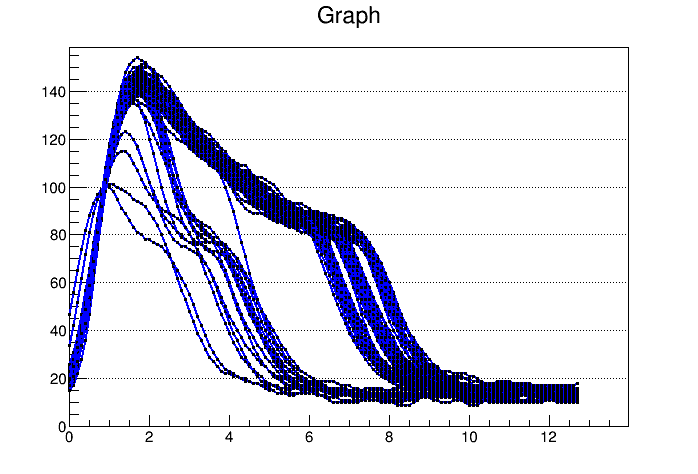
\includegraphics{../grafici/risultati/misura450.png}
 }%
 \caption{Grafico segnali a 450mb} 
 \label{gr:misura_450} 
\end{grafico}

\begin{grafico}
 \centering
 \resizebox{\textwidth}{!}{%
 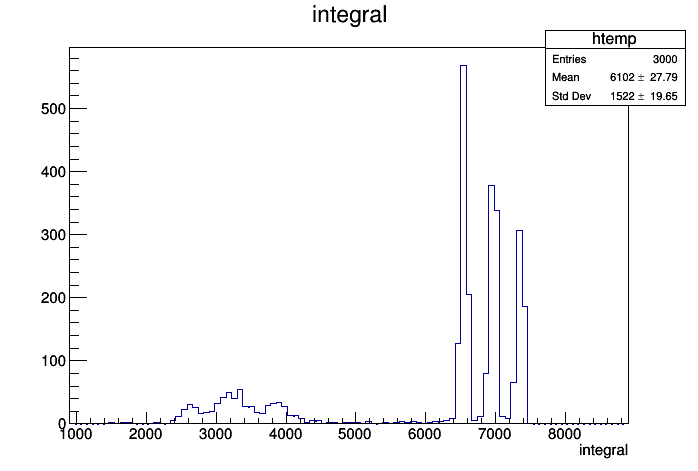
\includegraphics{../grafici/risultati/misura450_integral.png}
 }%
 \caption{Grafico integrale} 
 \label{gr:misura450_integral} 
\end{grafico}

 \begin{grafico}
 \centering
 \resizebox{\textwidth}{!}{%
 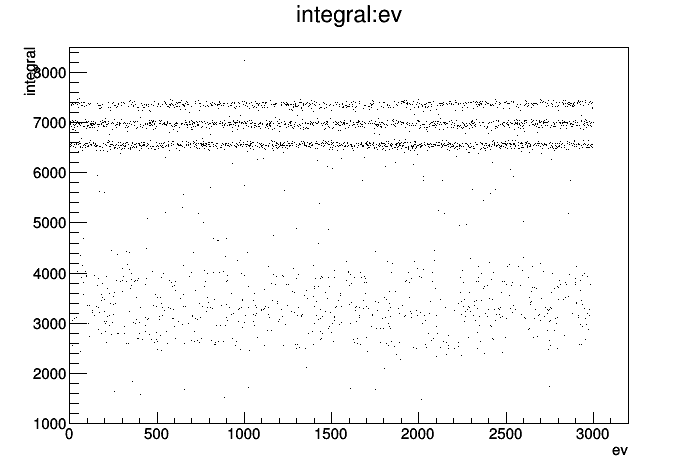
\includegraphics{../grafici/risultati/misura450_integral_ev.png}
 }%
 \caption{Grafico integral:ev} 
 \label{gr:misura450_integral_ev} 
\end{grafico}

 \begin{grafico}
 \centering
 \resizebox{\textwidth}{!}{%
 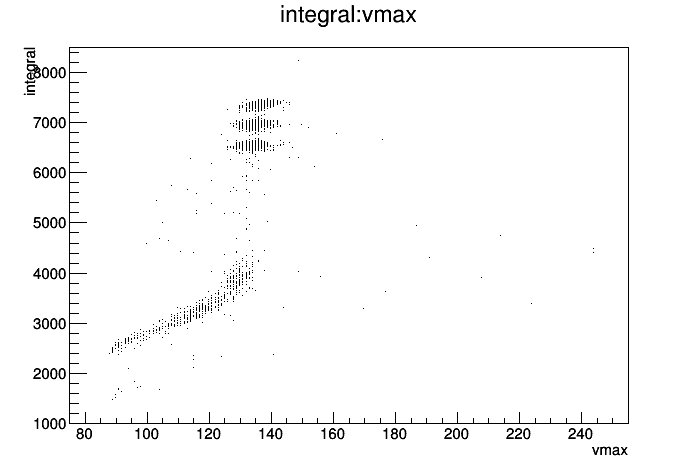
\includegraphics{../grafici/risultati/misura450_integral_vmax.png}
 }%
 \caption{Grafico integral:vmax} 
 \label{gr:misura450_integral_vmax} 
\end{grafico}

\begin{grafico}
 \centering
 \resizebox{\textwidth}{!}{%
 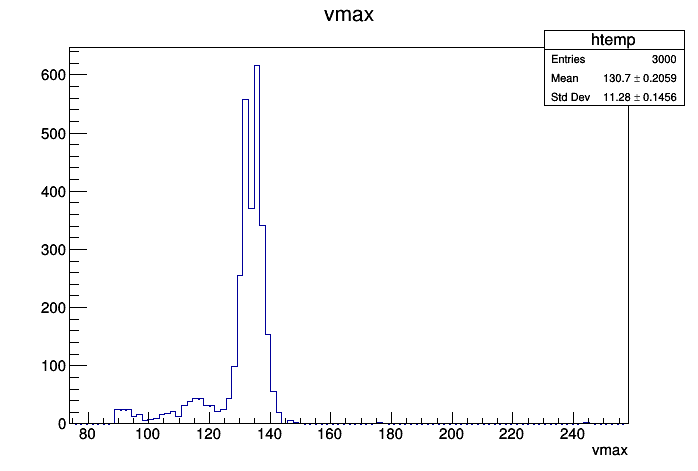
\includegraphics{../grafici/risultati/misura450_vmax.png}
 }%
 \caption{Grafico vmax} 
 \label{gr:misura450_vmax} 
\end{grafico}

 \begin{grafico}
 \centering
 \resizebox{\textwidth}{!}{%
 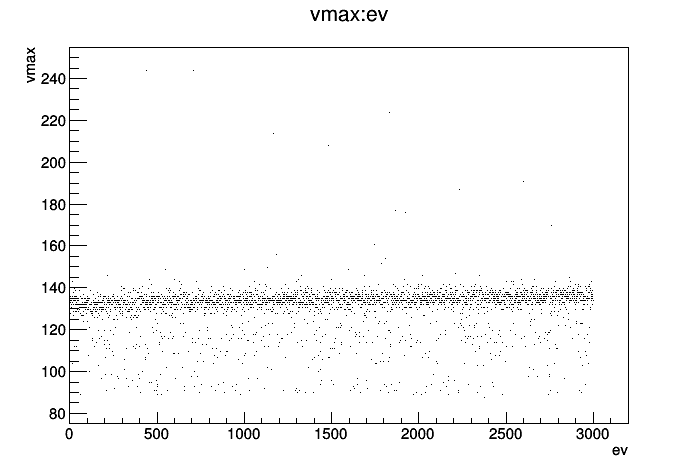
\includegraphics{../grafici/risultati/misura450_vmax_ev.png}
 }%
 \caption{Grafico vmax:ev} 
 \label{gr:misura450_vmax_ev} 
\end{grafico}

\FloatBarrier

\subsection{Misure a pressione 400mb}
\FloatBarrier

\begin{grafico}[H]
 \centering
 \resizebox{\textwidth}{!}{%
 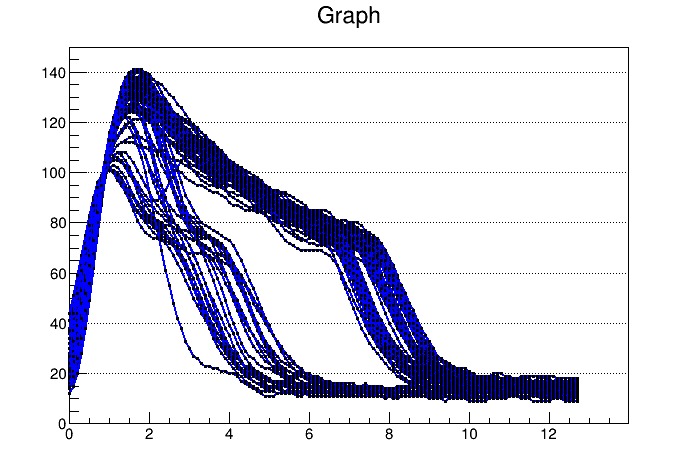
\includegraphics{../grafici/risultati/misura400.png}
 }%
 \caption{Grafico segnali a 400mb} 
 \label{gr:misura_400} 
\end{grafico}
\begin{grafico}
 \centering
 \resizebox{\textwidth}{!}{%
 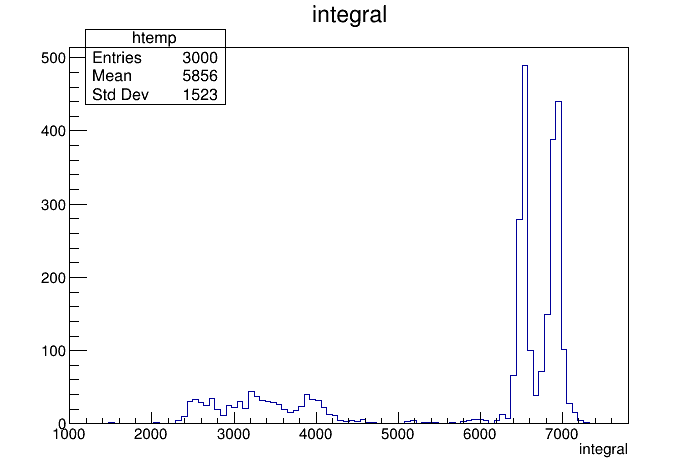
\includegraphics{../grafici/risultati/misura400_integral.png}
 }%
 \caption{Grafico integrale} 
 \label{gr:misura400_integral} 
\end{grafico}

 \begin{grafico}
 \centering
 \resizebox{\textwidth}{!}{%
 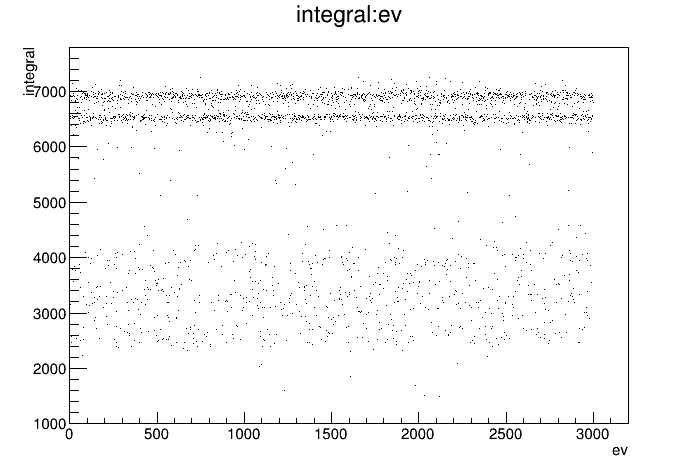
\includegraphics{../grafici/risultati/misura400_integral_ev.png}
 }%
 \caption{Grafico integral:ev} 
 \label{gr:misura400_integral_ev} 
\end{grafico}

 \begin{grafico}
 \centering
 \resizebox{\textwidth}{!}{%
 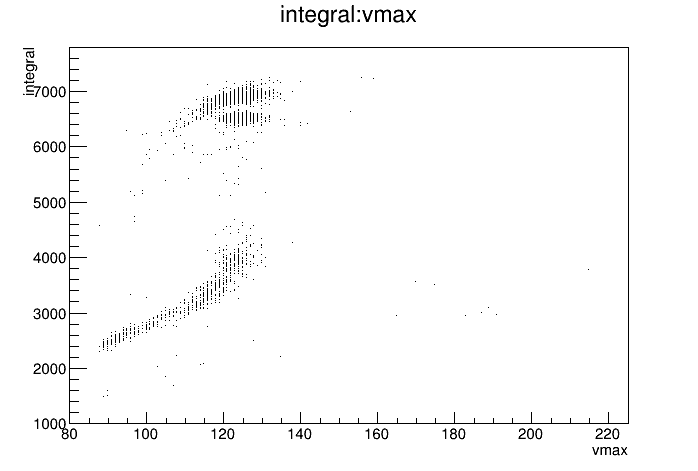
\includegraphics{../grafici/risultati/misura400_integral_vmax.png}
 }%
 \caption{Grafico integral:vmax} 
 \label{gr:misura400_integral_vmax} 
\end{grafico}

\begin{grafico}
 \centering
 \resizebox{\textwidth}{!}{%
 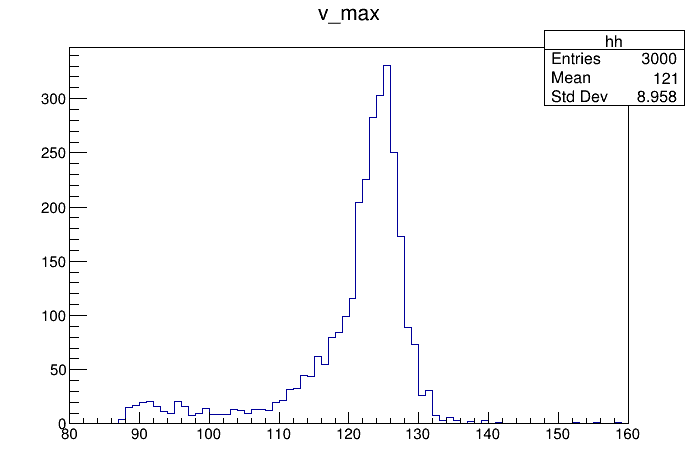
\includegraphics{../grafici/risultati/misura400_vmax.png}
 }%
 \caption{Grafico vmax} 
 \label{gr:misura400_vmax} 
\end{grafico}

 \begin{grafico}
 \centering
 \resizebox{\textwidth}{!}{%
 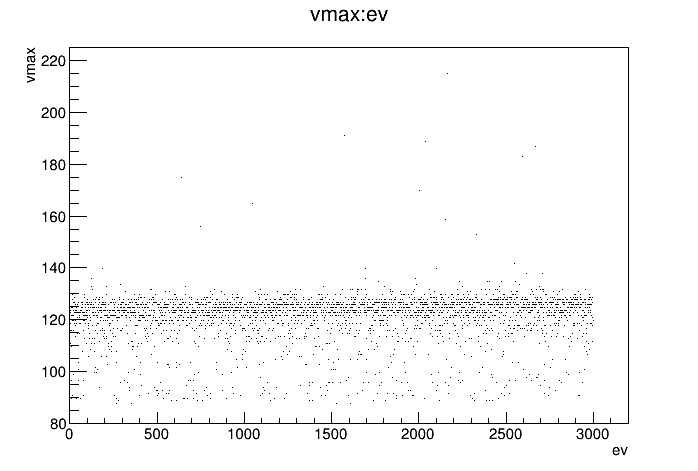
\includegraphics{../grafici/risultati/misura400_vmax_ev.png}
 }%
 \caption{Grafico vmax:ev} 
 \label{gr:misura400_vmax_ev} 
\end{grafico}

\FloatBarrier

\subsection{Misure a pressione 380mb}
\FloatBarrier

\begin{grafico}[H]
 \centering
 \resizebox{\textwidth}{!}{%
 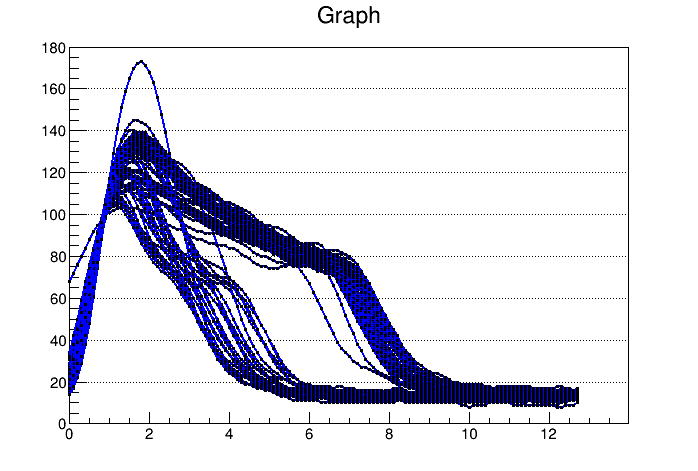
\includegraphics{../grafici/risultati/misura380.png}
 }%
 \caption{Grafico segnali a 380mb} 
 \label{gr:misura_380} 
\end{grafico}

\begin{grafico}[H]
 \centering
 \resizebox{\textwidth}{!}{%
 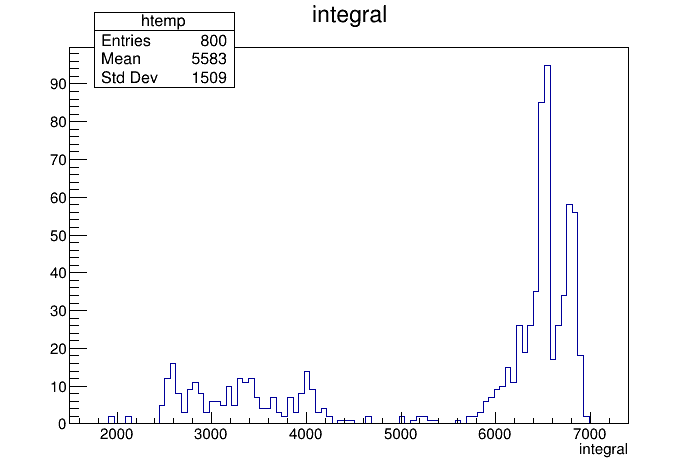
\includegraphics{../grafici/risultati/misura380_integral.png}
 }%
 \caption{Grafico integrale} 
 \label{gr:misura380_integral} 
\end{grafico}

 \begin{grafico}
 \centering
 \resizebox{\textwidth}{!}{%
 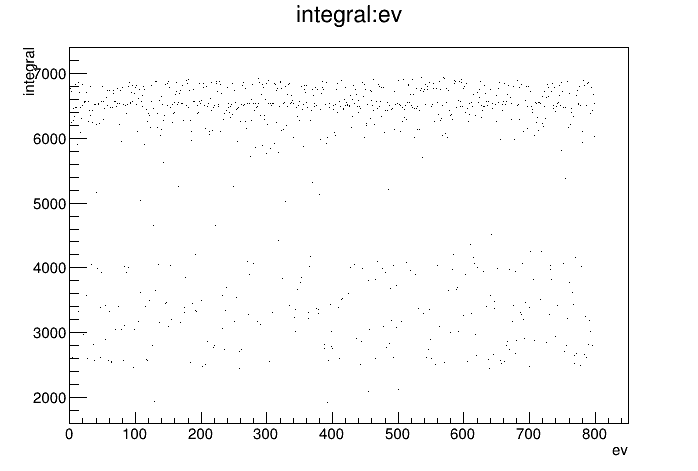
\includegraphics{../grafici/risultati/misura380_integral_ev.png}
 }%
 \caption{Grafico integral:ev} 
 \label{gr:misura380_integral_ev} 
\end{grafico}

 \begin{grafico}
 \centering
 \resizebox{\textwidth}{!}{%
 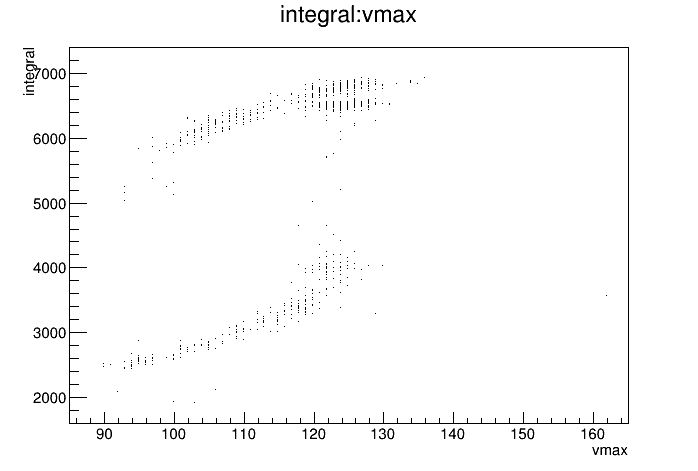
\includegraphics{../grafici/risultati/misura380_integral_vmax.png}
 }%
 \caption{Grafico integral:vmax} 
 \label{gr:misura380_integral_vmax} 
\end{grafico}

\begin{grafico}
 \centering
 \resizebox{\textwidth}{!}{%
 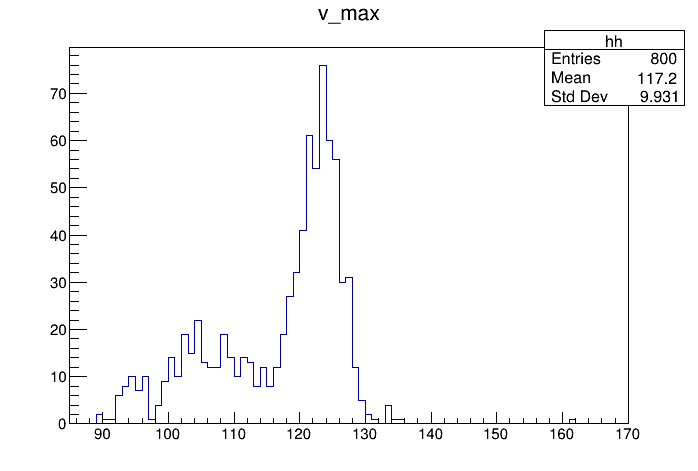
\includegraphics{../grafici/risultati/misura380_vmax.png}
 }%
 \caption{Grafico vmax} 
 \label{gr:misura380_vmax} 
\end{grafico}

 \begin{grafico}
 \centering
 \resizebox{\textwidth}{!}{%
 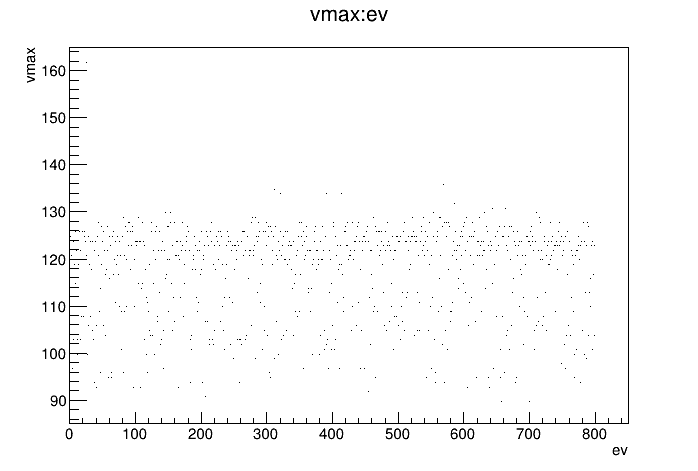
\includegraphics{../grafici/risultati/misura380_vmax_ev.png}
 }%
 \caption{Grafico vmax:ev} 
 \label{gr:misura380_vmax_ev} 
\end{grafico}


\FloatBarrier
\FloatBarrier

	%\subsection{Tabelle}

	\FloatBarrier
%\subsection{Tabelle dati}

\begin{tabella}
 \centering
 \begin{center}
\begin{tabulary}{\textwidth}{CC}
\toprule
 f(Hz) & A \\ \midrule
 10 & $1.01\pm0.03$   \\ \midrule
 30 & $1.01\pm0.03$  \\ \midrule
 100 & $1.01\pm0.03$  \\ \midrule
 300 & $1.01\pm0.03$  \\ \midrule
 1000 & $1.01\pm0.03$ \\ \midrule
 3000 & $1.00\pm0.03$   \\ \midrule
 10000 & $1.00\pm0.03$  \\ \midrule
 30000 & $1.01\pm0.03$  \\ \midrule
 100000 & $1.02\pm0.03$  \\ \midrule
 300000 & $1.08\pm0.04$  \\ \midrule
 800000 & $1.18\pm0.04$  \\ \midrule
 900000 & $1.05\pm0.03$  \\ \midrule
 1000000 & $0.90\pm0.03$ \\ \midrule
1130000 & $0.71\pm0.02$  \\ \midrule
1500000 & $0.39\pm0.01$  \\ \midrule
2000000 & $0.210\pm0.007$  \\ \midrule
3000000 & $0.090\pm0.003$  \\ \midrule
6000000 & $0.030\pm0.001$  \\ \midrule
 \bottomrule
\end{tabulary}
\end{center}


 
 \caption{Dati risposta in frequenza}
 \label{tab:tab_noninv_A1.tex}
\end{tabella}

\begin{tabella}
 \centering
  \begin{center}
\begin{tabulary}{\textwidth}{CC}
\toprule
f(Hz) & A  \\ \midrule
10 & 4.9$\pm$0.2  \\ \midrule
40 & 4.9$\pm$0.2  \\ \midrule
100 & 4.9$\pm$0.2  \\ \midrule
300 & 4.9$\pm$0.2  \\ \midrule
1000 & 4.9$\pm$0.2  \\ \midrule
3000 & 4.9$\pm$0.2  \\ \midrule
10000 & 4.9$\pm$0.2 \\ \midrule
30000 & 4.9$\pm$0.2  \\ \midrule
100000 & 4.8$\pm$0.2  \\ \midrule
300000 & 4.3$\pm$0.1  \\ \midrule
400000 & 4.0$\pm$0.1  \\ \midrule
515000 & 3.5$\pm$0.1   \\ \midrule
600000 & 3.2$\pm$0.1   \\ \midrule
1000000 & 2.02$\pm$0.07  \\ \midrule
3000000 & 0.44$\pm$0.01  \\ \midrule
5000000 & 0.170$\pm$0.006  \\ \midrule
 \bottomrule
\end{tabulary}
\end{center}



 
 \caption{Dati risposta in frequenza}
 \label{tab:tab_noninv_A5.tex}
\end{tabella}

\begin{tabella}
 \centering
 \begin{center}
\begin{tabulary}{\textwidth}{CC}
\toprule
f(Hz) & A   \\ \midrule
10 & 10.1$\pm$0.3  \\ \midrule
50 & 10.1$\pm$0.3  \\ \midrule
100 & 10.1$\pm$0.3  \\ \midrule
500 & 10.1$\pm$0.3  \\ \midrule
1000 & 10.1$\pm$0.3  \\ \midrule
5000 & 10.1$\pm$0.3  \\ \midrule
50000 & 9.4$\pm$0.3  \\ \midrule
100000 & 9.2$\pm$0.3  \\ \midrule
200000 & 7.5$\pm$0.3  \\ \midrule
211000 & 7.1$\pm$0.2  \\ \midrule
215000 & 7.1$\pm$0.2  \\ \midrule
220000 & 7.1$\pm$0.2  \\ \midrule
230000 & 6.9$\pm$0.2  \\ \midrule
250000 & 6.5$\pm$0.2  \\ \midrule
300000 & 5.9$\pm$0.2  \\ \midrule
400000 & 4.7$\pm$0.2  \\ \midrule
500000 & 3.69$\pm$0.1  \\ \midrule
1000000 & 1.57$\pm$0.05  \\ \midrule
5000000 & 0.110$\pm$0.003  \\ \midrule
\bottomrule
\end{tabulary}
\end{center} 
 \caption{Dati risposta in frequenza}
 \label{tab:tab_noninv_A10.tex}
\end{tabella}

\FloatBarrier



	%\clearpage
	%\subsection{Grafici}
	%% \begin{grafico} \centering \input{../gnuplot/immagini/02_graph_1.tex} \caption{Grafico 02_graph_1.tex} \label{gr:02_graph_1.tex} \end{grafico}
% \begin{grafico} \centering \input{../gnuplot/immagini/02_graph_3.tex} \caption{Grafico 02_graph_3.tex} \label{gr:02_graph_3.tex} \end{grafico}
% \begin{grafico} \centering \input{../gnuplot/immagini/02_graph_4.tex} \caption{Grafico 02_graph_4.tex} \label{gr:02_graph_4.tex} \end{grafico}


%\clearpage
%\begin{multicols}{2}

	
\section{Discussioni e conclusioni}
	E' stata fatta la simulazione per la risposta in frequenza utilizzando Spice, con l'accortezza di scaricare la libreria del componente
dal sito della Texas Instrument.
I  \autoref{gr:sim_a5.tex} e \autoref{gr:sim_a10.tex} mostrano il confronto della simulazione con 
i dati sperimentali e mostrano un buon accordo tra i dati e la simulazione.
Nel \autoref{gr:sim_a1.tex}, relativo all'ampificazione A=1, si nota una deviazione dei dati sperimentali dovuta alla risonanza,
causata dalle induttanze parassite nel circuito reale, che comportano lo spostamento verso le basse frequenze del polo.

\begin{grafico}
 \centering
 \resizebox{\textwidth}{!}{%
 \begin{tikzpicture}
\pgfdeclareplotmark{cross} {
\pgfpathmoveto{\pgfpoint{-0.3\pgfplotmarksize}{\pgfplotmarksize}}
\pgfpathlineto{\pgfpoint{+0.3\pgfplotmarksize}{\pgfplotmarksize}}
\pgfpathlineto{\pgfpoint{+0.3\pgfplotmarksize}{0.3\pgfplotmarksize}}
\pgfpathlineto{\pgfpoint{+1\pgfplotmarksize}{0.3\pgfplotmarksize}}
\pgfpathlineto{\pgfpoint{+1\pgfplotmarksize}{-0.3\pgfplotmarksize}}
\pgfpathlineto{\pgfpoint{+0.3\pgfplotmarksize}{-0.3\pgfplotmarksize}}
\pgfpathlineto{\pgfpoint{+0.3\pgfplotmarksize}{-1.\pgfplotmarksize}}
\pgfpathlineto{\pgfpoint{-0.3\pgfplotmarksize}{-1.\pgfplotmarksize}}
\pgfpathlineto{\pgfpoint{-0.3\pgfplotmarksize}{-0.3\pgfplotmarksize}}
\pgfpathlineto{\pgfpoint{-1.\pgfplotmarksize}{-0.3\pgfplotmarksize}}
\pgfpathlineto{\pgfpoint{-1.\pgfplotmarksize}{0.3\pgfplotmarksize}}
\pgfpathlineto{\pgfpoint{-0.3\pgfplotmarksize}{0.3\pgfplotmarksize}}
\pgfpathclose
\pgfusepathqstroke
}
\pgfdeclareplotmark{cross*} {
\pgfpathmoveto{\pgfpoint{-0.3\pgfplotmarksize}{\pgfplotmarksize}}
\pgfpathlineto{\pgfpoint{+0.3\pgfplotmarksize}{\pgfplotmarksize}}
\pgfpathlineto{\pgfpoint{+0.3\pgfplotmarksize}{0.3\pgfplotmarksize}}
\pgfpathlineto{\pgfpoint{+1\pgfplotmarksize}{0.3\pgfplotmarksize}}
\pgfpathlineto{\pgfpoint{+1\pgfplotmarksize}{-0.3\pgfplotmarksize}}
\pgfpathlineto{\pgfpoint{+0.3\pgfplotmarksize}{-0.3\pgfplotmarksize}}
\pgfpathlineto{\pgfpoint{+0.3\pgfplotmarksize}{-1.\pgfplotmarksize}}
\pgfpathlineto{\pgfpoint{-0.3\pgfplotmarksize}{-1.\pgfplotmarksize}}
\pgfpathlineto{\pgfpoint{-0.3\pgfplotmarksize}{-0.3\pgfplotmarksize}}
\pgfpathlineto{\pgfpoint{-1.\pgfplotmarksize}{-0.3\pgfplotmarksize}}
\pgfpathlineto{\pgfpoint{-1.\pgfplotmarksize}{0.3\pgfplotmarksize}}
\pgfpathlineto{\pgfpoint{-0.3\pgfplotmarksize}{0.3\pgfplotmarksize}}
\pgfpathclose
\pgfusepathqfillstroke
}
\pgfdeclareplotmark{newstar} {
\pgfpathmoveto{\pgfqpoint{0pt}{\pgfplotmarksize}}
\pgfpathlineto{\pgfqpointpolar{44}{0.5\pgfplotmarksize}}
\pgfpathlineto{\pgfqpointpolar{18}{\pgfplotmarksize}}
\pgfpathlineto{\pgfqpointpolar{-20}{0.5\pgfplotmarksize}}
\pgfpathlineto{\pgfqpointpolar{-54}{\pgfplotmarksize}}
\pgfpathlineto{\pgfqpointpolar{-90}{0.5\pgfplotmarksize}}
\pgfpathlineto{\pgfqpointpolar{234}{\pgfplotmarksize}}
\pgfpathlineto{\pgfqpointpolar{198}{0.5\pgfplotmarksize}}
\pgfpathlineto{\pgfqpointpolar{162}{\pgfplotmarksize}}
\pgfpathlineto{\pgfqpointpolar{134}{0.5\pgfplotmarksize}}
\pgfpathclose
\pgfusepathqstroke
}
\pgfdeclareplotmark{newstar*} {
\pgfpathmoveto{\pgfqpoint{0pt}{\pgfplotmarksize}}
\pgfpathlineto{\pgfqpointpolar{44}{0.5\pgfplotmarksize}}
\pgfpathlineto{\pgfqpointpolar{18}{\pgfplotmarksize}}
\pgfpathlineto{\pgfqpointpolar{-20}{0.5\pgfplotmarksize}}
\pgfpathlineto{\pgfqpointpolar{-54}{\pgfplotmarksize}}
\pgfpathlineto{\pgfqpointpolar{-90}{0.5\pgfplotmarksize}}
\pgfpathlineto{\pgfqpointpolar{234}{\pgfplotmarksize}}
\pgfpathlineto{\pgfqpointpolar{198}{0.5\pgfplotmarksize}}
\pgfpathlineto{\pgfqpointpolar{162}{\pgfplotmarksize}}
\pgfpathlineto{\pgfqpointpolar{134}{0.5\pgfplotmarksize}}
\pgfpathclose
\pgfusepathqfillstroke
}
\definecolor{c}{rgb}{1,1,1};
\draw [color=c, fill=c] (0,0) rectangle (20,13.4957);
\draw [color=c, fill=c] (2,1.34957) rectangle (18,12.1461);
\definecolor{c}{rgb}{0,0,0};
\draw [c,line width=0.9] (2,1.34957) -- (2,12.1461) -- (18,12.1461) -- (18,1.34957) -- (2,1.34957);
\definecolor{c}{rgb}{1,1,1};
\draw [color=c, fill=c] (2,1.34957) rectangle (18,12.1461);
\definecolor{c}{rgb}{0,0,0};
\draw [c,line width=0.9] (2,1.34957) -- (2,12.1461) -- (18,12.1461) -- (18,1.34957) -- (2,1.34957);
\draw [c,line width=0.9] (2,1.34957) -- (18,1.34957);
\draw [c,dotted,line width=0.9] (2.09053,12.1461) -- (2.09053,1.34957);
\draw [c,dotted,line width=0.9] (4.06897,12.1461) -- (4.06897,1.34957);
\draw [c,dotted,line width=0.9] (6.04742,12.1461) -- (6.04742,1.34957);
\draw [c,dotted,line width=0.9] (8.02587,12.1461) -- (8.02587,1.34957);
\draw [c,dotted,line width=0.9] (10.0043,12.1461) -- (10.0043,1.34957);
\draw [c,dotted,line width=0.9] (11.9828,12.1461) -- (11.9828,1.34957);
\draw [c,dotted,line width=0.9] (13.9612,12.1461) -- (13.9612,1.34957);
\draw [c,dotted,line width=0.9] (15.9397,12.1461) -- (15.9397,1.34957);
\draw [c,dotted,line width=0.9] (17.9181,12.1461) -- (17.9181,1.34957);
\draw [c,line width=0.9] (2,1.34957) -- (2,12.1461);
\draw [c,dotted,line width=0.9] (18,2.19381) -- (2,2.19381);
\draw [c,dotted,line width=0.9] (18,2.82754) -- (2,2.82754);
\draw [c,dotted,line width=0.9] (18,3.27717) -- (2,3.27717);
\draw [c,dotted,line width=0.9] (18,3.62594) -- (2,3.62594);
\draw [c,dotted,line width=0.9] (18,3.9109) -- (2,3.9109);
\draw [c,dotted,line width=0.9] (18,4.15183) -- (2,4.15183);
\draw [c,dotted,line width=0.9] (18,4.36054) -- (2,4.36054);
\draw [c,dotted,line width=0.9] (18,4.54463) -- (2,4.54463);
\draw [c,dotted,line width=0.9] (18,4.7093) -- (2,4.7093);
\draw [c,dotted,line width=0.9] (18,5.79266) -- (2,5.79266);
\draw [c,dotted,line width=0.9] (18,6.42639) -- (2,6.42639);
\draw [c,dotted,line width=0.9] (18,6.87603) -- (2,6.87603);
\draw [c,dotted,line width=0.9] (18,7.22479) -- (2,7.22479);
\draw [c,dotted,line width=0.9] (18,7.50975) -- (2,7.50975);
\draw [c,dotted,line width=0.9] (18,7.75068) -- (2,7.75068);
\draw [c,dotted,line width=0.9] (18,7.95939) -- (2,7.95939);
\draw [c,dotted,line width=0.9] (18,8.14348) -- (2,8.14348);
\draw [c,dotted,line width=0.9] (18,8.30815) -- (2,8.30815);
\draw [c,dotted,line width=0.9] (18,9.39151) -- (2,9.39151);
\draw [c,dotted,line width=0.9] (18,10.0252) -- (2,10.0252);
\draw [c,dotted,line width=0.9] (18,10.4749) -- (2,10.4749);
\draw [c,dotted,line width=0.9] (18,10.8236) -- (2,10.8236);
\draw [c,dotted,line width=0.9] (18,11.1086) -- (2,11.1086);
\draw [c,dotted,line width=0.9] (18,11.3495) -- (2,11.3495);
\draw [c,dotted,line width=0.9] (18,11.5582) -- (2,11.5582);
\draw [c,dotted,line width=0.9] (18,11.7423) -- (2,11.7423);
\draw [c,dotted,line width=0.9] (18,11.907) -- (2,11.907);
\draw [c,line width=0.9] (2,1.34957) -- (18,1.34957);
\draw [c,line width=0.9] (2.09053,1.67347) -- (2.09053,1.34957);
\draw [anchor=base] (2.09053,0.73889) node[scale=1.01821, color=c, rotate=0]{10};
\draw [c,line width=0.9] (2.6861,1.51152) -- (2.6861,1.34957);
\draw [c,line width=0.9] (3.03449,1.51152) -- (3.03449,1.34957);
\draw [c,line width=0.9] (3.28167,1.51152) -- (3.28167,1.34957);
\draw [c,line width=0.9] (3.4734,1.51152) -- (3.4734,1.34957);
\draw [c,line width=0.9] (3.63006,1.51152) -- (3.63006,1.34957);
\draw [c,line width=0.9] (3.76251,1.51152) -- (3.76251,1.34957);
\draw [c,line width=0.9] (3.87724,1.51152) -- (3.87724,1.34957);
\draw [c,line width=0.9] (3.97845,1.51152) -- (3.97845,1.34957);
\draw [c,line width=0.9] (4.06897,1.67347) -- (4.06897,1.34957);
\draw [anchor=base] (4.06897,0.73889) node[scale=1.01821, color=c, rotate=0]{$10^{2}$};
\draw [c,line width=0.9] (4.66455,1.51152) -- (4.66455,1.34957);
\draw [c,line width=0.9] (5.01293,1.51152) -- (5.01293,1.34957);
\draw [c,line width=0.9] (5.26012,1.51152) -- (5.26012,1.34957);
\draw [c,line width=0.9] (5.45185,1.51152) -- (5.45185,1.34957);
\draw [c,line width=0.9] (5.60851,1.51152) -- (5.60851,1.34957);
\draw [c,line width=0.9] (5.74096,1.51152) -- (5.74096,1.34957);
\draw [c,line width=0.9] (5.85569,1.51152) -- (5.85569,1.34957);
\draw [c,line width=0.9] (5.95689,1.51152) -- (5.95689,1.34957);
\draw [c,line width=0.9] (6.04742,1.67347) -- (6.04742,1.34957);
\draw [anchor=base] (6.04742,0.73889) node[scale=1.01821, color=c, rotate=0]{$10^{3}$};
\draw [c,line width=0.9] (6.64299,1.51152) -- (6.64299,1.34957);
\draw [c,line width=0.9] (6.99138,1.51152) -- (6.99138,1.34957);
\draw [c,line width=0.9] (7.23857,1.51152) -- (7.23857,1.34957);
\draw [c,line width=0.9] (7.4303,1.51152) -- (7.4303,1.34957);
\draw [c,line width=0.9] (7.58695,1.51152) -- (7.58695,1.34957);
\draw [c,line width=0.9] (7.7194,1.51152) -- (7.7194,1.34957);
\draw [c,line width=0.9] (7.83414,1.51152) -- (7.83414,1.34957);
\draw [c,line width=0.9] (7.93534,1.51152) -- (7.93534,1.34957);
\draw [c,line width=0.9] (8.02587,1.67347) -- (8.02587,1.34957);
\draw [anchor=base] (8.02587,0.73889) node[scale=1.01821, color=c, rotate=0]{$10^{4}$};
\draw [c,line width=0.9] (8.62144,1.51152) -- (8.62144,1.34957);
\draw [c,line width=0.9] (8.96983,1.51152) -- (8.96983,1.34957);
\draw [c,line width=0.9] (9.21701,1.51152) -- (9.21701,1.34957);
\draw [c,line width=0.9] (9.40874,1.51152) -- (9.40874,1.34957);
\draw [c,line width=0.9] (9.5654,1.51152) -- (9.5654,1.34957);
\draw [c,line width=0.9] (9.69785,1.51152) -- (9.69785,1.34957);
\draw [c,line width=0.9] (9.81259,1.51152) -- (9.81259,1.34957);
\draw [c,line width=0.9] (9.91379,1.51152) -- (9.91379,1.34957);
\draw [c,line width=0.9] (10.0043,1.67347) -- (10.0043,1.34957);
\draw [anchor=base] (10.0043,0.73889) node[scale=1.01821, color=c, rotate=0]{$10^{5}$};
\draw [c,line width=0.9] (10.5999,1.51152) -- (10.5999,1.34957);
\draw [c,line width=0.9] (10.9483,1.51152) -- (10.9483,1.34957);
\draw [c,line width=0.9] (11.1955,1.51152) -- (11.1955,1.34957);
\draw [c,line width=0.9] (11.3872,1.51152) -- (11.3872,1.34957);
\draw [c,line width=0.9] (11.5438,1.51152) -- (11.5438,1.34957);
\draw [c,line width=0.9] (11.6763,1.51152) -- (11.6763,1.34957);
\draw [c,line width=0.9] (11.791,1.51152) -- (11.791,1.34957);
\draw [c,line width=0.9] (11.8922,1.51152) -- (11.8922,1.34957);
\draw [c,line width=0.9] (11.9828,1.67347) -- (11.9828,1.34957);
\draw [anchor=base] (11.9828,0.73889) node[scale=1.01821, color=c, rotate=0]{$10^{6}$};
\draw [c,line width=0.9] (12.5783,1.51152) -- (12.5783,1.34957);
\draw [c,line width=0.9] (12.9267,1.51152) -- (12.9267,1.34957);
\draw [c,line width=0.9] (13.1739,1.51152) -- (13.1739,1.34957);
\draw [c,line width=0.9] (13.3656,1.51152) -- (13.3656,1.34957);
\draw [c,line width=0.9] (13.5223,1.51152) -- (13.5223,1.34957);
\draw [c,line width=0.9] (13.6547,1.51152) -- (13.6547,1.34957);
\draw [c,line width=0.9] (13.7695,1.51152) -- (13.7695,1.34957);
\draw [c,line width=0.9] (13.8707,1.51152) -- (13.8707,1.34957);
\draw [c,line width=0.9] (13.9612,1.67347) -- (13.9612,1.34957);
\draw [anchor=base] (13.9612,0.73889) node[scale=1.01821, color=c, rotate=0]{$10^{7}$};
\draw [c,line width=0.9] (14.5568,1.51152) -- (14.5568,1.34957);
\draw [c,line width=0.9] (14.9052,1.51152) -- (14.9052,1.34957);
\draw [c,line width=0.9] (15.1524,1.51152) -- (15.1524,1.34957);
\draw [c,line width=0.9] (15.3441,1.51152) -- (15.3441,1.34957);
\draw [c,line width=0.9] (15.5007,1.51152) -- (15.5007,1.34957);
\draw [c,line width=0.9] (15.6332,1.51152) -- (15.6332,1.34957);
\draw [c,line width=0.9] (15.7479,1.51152) -- (15.7479,1.34957);
\draw [c,line width=0.9] (15.8491,1.51152) -- (15.8491,1.34957);
\draw [c,line width=0.9] (15.9397,1.67347) -- (15.9397,1.34957);
\draw [anchor=base] (15.9397,0.73889) node[scale=1.01821, color=c, rotate=0]{$10^{8}$};
\draw [c,line width=0.9] (16.5352,1.51152) -- (16.5352,1.34957);
\draw [c,line width=0.9] (16.8836,1.51152) -- (16.8836,1.34957);
\draw [c,line width=0.9] (17.1308,1.51152) -- (17.1308,1.34957);
\draw [c,line width=0.9] (17.3225,1.51152) -- (17.3225,1.34957);
\draw [c,line width=0.9] (17.4792,1.51152) -- (17.4792,1.34957);
\draw [c,line width=0.9] (17.6116,1.51152) -- (17.6116,1.34957);
\draw [c,line width=0.9] (17.7264,1.51152) -- (17.7264,1.34957);
\draw [c,line width=0.9] (17.8276,1.51152) -- (17.8276,1.34957);
\draw [c,line width=0.9] (17.9181,1.67347) -- (17.9181,1.34957);
\draw [anchor=base] (17.9181,0.73889) node[scale=1.01821, color=c, rotate=0]{$10^{9}$};
\draw [c,line width=0.9] (2,1.34957) -- (2,12.1461);
\draw [c,line width=0.9] (2.24,2.19381) -- (2,2.19381);
\draw [c,line width=0.9] (2.24,2.82754) -- (2,2.82754);
\draw [c,line width=0.9] (2.24,3.27717) -- (2,3.27717);
\draw [c,line width=0.9] (2.24,3.62594) -- (2,3.62594);
\draw [c,line width=0.9] (2.24,3.9109) -- (2,3.9109);
\draw [c,line width=0.9] (2.24,4.15183) -- (2,4.15183);
\draw [c,line width=0.9] (2.24,4.36054) -- (2,4.36054);
\draw [c,line width=0.9] (2.24,4.54463) -- (2,4.54463);
\draw [c,line width=0.9] (2.48,4.7093) -- (2,4.7093);
\draw [anchor= east] (1.844,4.7093) node[scale=1.01821, color=c, rotate=0]{$10^{-2}$};
\draw [c,line width=0.9] (2.24,5.79266) -- (2,5.79266);
\draw [c,line width=0.9] (2.24,6.42639) -- (2,6.42639);
\draw [c,line width=0.9] (2.24,6.87603) -- (2,6.87603);
\draw [c,line width=0.9] (2.24,7.22479) -- (2,7.22479);
\draw [c,line width=0.9] (2.24,7.50975) -- (2,7.50975);
\draw [c,line width=0.9] (2.24,7.75068) -- (2,7.75068);
\draw [c,line width=0.9] (2.24,7.95939) -- (2,7.95939);
\draw [c,line width=0.9] (2.24,8.14348) -- (2,8.14348);
\draw [c,line width=0.9] (2.48,8.30815) -- (2,8.30815);
\draw [anchor= east] (1.844,8.30815) node[scale=1.01821, color=c, rotate=0]{$10^{-1}$};
\draw [c,line width=0.9] (2.24,9.39151) -- (2,9.39151);
\draw [c,line width=0.9] (2.24,10.0252) -- (2,10.0252);
\draw [c,line width=0.9] (2.24,10.4749) -- (2,10.4749);
\draw [c,line width=0.9] (2.24,10.8236) -- (2,10.8236);
\draw [c,line width=0.9] (2.24,11.1086) -- (2,11.1086);
\draw [c,line width=0.9] (2.24,11.3495) -- (2,11.3495);
\draw [c,line width=0.9] (2.24,11.5582) -- (2,11.5582);
\draw [c,line width=0.9] (2.24,11.7423) -- (2,11.7423);
\draw [c,line width=0.9] (2.48,11.907) -- (2,11.907);
\draw [anchor= east] (1.844,11.907) node[scale=1.01821, color=c, rotate=0]{1};
\definecolor{c}{rgb}{0,0,1};
\draw [c,line width=0.9] (2.09053,11.9972) -- (2.28837,11.9972) -- (2.48622,11.9972) -- (2.68406,11.9972) -- (2.88191,11.9972) -- (3.07975,11.9972) -- (3.2776,11.9972) -- (3.47544,11.9972) -- (3.67329,11.9972) -- (3.87113,11.9972) --
 (4.06898,11.9972) -- (4.26682,11.9972) -- (4.46467,11.9972) -- (4.66251,11.9972) -- (4.86035,11.9972) -- (5.0582,11.9972) -- (5.25604,11.9972) -- (5.45389,11.9972) -- (5.65173,11.9972) -- (5.84958,11.9972) -- (6.04742,11.9972) -- (6.24527,11.9972)
 -- (6.44311,11.9972) -- (6.64096,11.9972) -- (6.8388,11.9972) -- (7.03665,11.9972) -- (7.23449,11.9972) -- (7.43234,11.9972) -- (7.63018,11.9972) -- (7.82803,11.9972) -- (8.02587,11.9972) -- (8.22371,11.9971) -- (8.42156,11.9971) -- (8.6194,11.9971)
 -- (8.81725,11.9971) -- (9.01509,11.997) -- (9.21294,11.997) -- (9.41078,11.9969) -- (9.60863,11.9967) -- (9.80647,11.9964) -- (10.0043,11.9959) -- (10.2022,11.9952) -- (10.4,11.9941) -- (10.5979,11.9922) -- (10.7957,11.9894) -- (10.9935,11.9848) --
 (11.1914,11.9776) -- (11.3892,11.9663) -- (11.5871,11.9484) -- (11.7849,11.9204) -- (11.9828,11.8768) -- (12.1806,11.8094) -- (12.3785,11.707) -- (12.5763,11.5551) -- (12.7741,11.3375) -- (12.972,11.0399) -- (13.1698,10.655) -- (13.3677,10.1858) --
 (13.5655,9.64421) -- (13.7634,9.04617) -- (13.9612,8.40724) -- (14.1591,7.74017) -- (14.3569,7.05434) -- (14.5547,6.35626) -- (14.7526,5.65028) -- (14.9504,4.93926) -- (15.1483,4.22503) -- (15.3461,3.50876) -- (15.544,2.7912) -- (15.7418,2.07283) --
 (15.9397,1.35394) -- (15.9409,1.34957);
\definecolor{c}{rgb}{0,0,0};
\foreach \P in {(2.09053,11.9972), (2.28837,11.9972), (2.48622,11.9972), (2.68406,11.9972), (2.88191,11.9972), (3.07975,11.9972), (3.2776,11.9972), (3.47544,11.9972), (3.67329,11.9972), (3.87113,11.9972), (4.06898,11.9972), (4.26682,11.9972),
 (4.46467,11.9972), (4.66251,11.9972), (4.86035,11.9972), (5.0582,11.9972), (5.25604,11.9972), (5.45389,11.9972), (5.65173,11.9972), (5.84958,11.9972), (6.04742,11.9972), (6.24527,11.9972), (6.44311,11.9972), (6.64096,11.9972), (6.8388,11.9972),
 (7.03665,11.9972), (7.23449,11.9972), (7.43234,11.9972), (7.63018,11.9972), (7.82803,11.9972), (8.02587,11.9972), (8.22371,11.9971), (8.42156,11.9971), (8.6194,11.9971), (8.81725,11.9971), (9.01509,11.997), (9.21294,11.997), (9.41078,11.9969),
 (9.60863,11.9967), (9.80647,11.9964), (10.0043,11.9959), (10.2022,11.9952), (10.4,11.9941), (10.5979,11.9922), (10.7957,11.9894), (10.9935,11.9848), (11.1914,11.9776), (11.3892,11.9663), (11.5871,11.9484), (11.7849,11.9204), (11.9828,11.8768),
 (12.1806,11.8094), (12.3785,11.707), (12.5763,11.5551), (12.7741,11.3375), (12.972,11.0399), (13.1698,10.655), (13.3677,10.1858), (13.5655,9.64421), (13.7634,9.04617), (13.9612,8.40724), (14.1591,7.74017), (14.3569,7.05434), (14.5547,6.35626),
 (14.7526,5.65028), (14.9504,4.93926), (15.1483,4.22503), (15.3461,3.50876), (15.544,2.7912), (15.7418,2.07283), (15.9397,1.35394)}{\draw[mark options={color=c,fill=c},mark size=2.402402pt,mark=*,mark size=1pt] plot coordinates {\P};}
\draw (8.45788,13.0156) node[scale=1.27276, color=c, rotate=0]{Confronto tra dati e simulazione};
\definecolor{c}{rgb}{1,0,0};
\draw [c,line width=0.9] (2.09053,11.9226) -- (3.03449,11.9226) -- (4.06898,11.9226) -- (5.01294,11.9226) -- (6.04742,11.9226) -- (6.99138,11.907) -- (8.02587,11.907) -- (8.96983,11.9226) -- (10.0043,11.938) -- (10.9483,12.0273) -- (11.6719,12.1461);
\draw [c,line width=0.9] (11.8019,12.1461) -- (11.8922,11.9833);
\draw [c,line width=0.9] (11.8922,11.9833) -- (11.9828,11.7423) -- (12.0878,11.3717) -- (12.3209,10.4585) -- (12.5501,9.48424) -- (12.9267,8.14348) -- (13.5223,6.42639);
\definecolor{c}{rgb}{0.573333,0,1};
\foreach \P in {(2.09053,11.9226), (3.03449,11.9226), (4.06898,11.9226), (5.01294,11.9226), (6.04742,11.9226), (6.99138,11.907), (8.02587,11.907), (8.96983,11.9226), (10.0043,11.938), (10.9483,12.0273)}{\draw[mark options={color=c,fill=c},mark
 size=1.201201pt,mark=o] plot coordinates {\P};}
\foreach \P in {(11.8922,11.9833), (11.9828,11.7423), (12.0878,11.3717), (12.3209,10.4585), (12.5501,9.48424), (12.9267,8.14348), (13.5223,6.42639)}{\draw[mark options={color=c,fill=c},mark size=1.201201pt,mark=o] plot coordinates {\P};}
\end{tikzpicture}

 }%
 \caption{Risposta in frequenza con Spice confrontata coi dati sperimentali (A=1)} 
 \label{gr:sim_a1.tex} 
\end{grafico}

\begin{grafico}
 \centering
 \resizebox{\textwidth}{!}{%
 \begin{tikzpicture}
\pgfdeclareplotmark{cross} {
\pgfpathmoveto{\pgfpoint{-0.3\pgfplotmarksize}{\pgfplotmarksize}}
\pgfpathlineto{\pgfpoint{+0.3\pgfplotmarksize}{\pgfplotmarksize}}
\pgfpathlineto{\pgfpoint{+0.3\pgfplotmarksize}{0.3\pgfplotmarksize}}
\pgfpathlineto{\pgfpoint{+1\pgfplotmarksize}{0.3\pgfplotmarksize}}
\pgfpathlineto{\pgfpoint{+1\pgfplotmarksize}{-0.3\pgfplotmarksize}}
\pgfpathlineto{\pgfpoint{+0.3\pgfplotmarksize}{-0.3\pgfplotmarksize}}
\pgfpathlineto{\pgfpoint{+0.3\pgfplotmarksize}{-1.\pgfplotmarksize}}
\pgfpathlineto{\pgfpoint{-0.3\pgfplotmarksize}{-1.\pgfplotmarksize}}
\pgfpathlineto{\pgfpoint{-0.3\pgfplotmarksize}{-0.3\pgfplotmarksize}}
\pgfpathlineto{\pgfpoint{-1.\pgfplotmarksize}{-0.3\pgfplotmarksize}}
\pgfpathlineto{\pgfpoint{-1.\pgfplotmarksize}{0.3\pgfplotmarksize}}
\pgfpathlineto{\pgfpoint{-0.3\pgfplotmarksize}{0.3\pgfplotmarksize}}
\pgfpathclose
\pgfusepathqstroke
}
\pgfdeclareplotmark{cross*} {
\pgfpathmoveto{\pgfpoint{-0.3\pgfplotmarksize}{\pgfplotmarksize}}
\pgfpathlineto{\pgfpoint{+0.3\pgfplotmarksize}{\pgfplotmarksize}}
\pgfpathlineto{\pgfpoint{+0.3\pgfplotmarksize}{0.3\pgfplotmarksize}}
\pgfpathlineto{\pgfpoint{+1\pgfplotmarksize}{0.3\pgfplotmarksize}}
\pgfpathlineto{\pgfpoint{+1\pgfplotmarksize}{-0.3\pgfplotmarksize}}
\pgfpathlineto{\pgfpoint{+0.3\pgfplotmarksize}{-0.3\pgfplotmarksize}}
\pgfpathlineto{\pgfpoint{+0.3\pgfplotmarksize}{-1.\pgfplotmarksize}}
\pgfpathlineto{\pgfpoint{-0.3\pgfplotmarksize}{-1.\pgfplotmarksize}}
\pgfpathlineto{\pgfpoint{-0.3\pgfplotmarksize}{-0.3\pgfplotmarksize}}
\pgfpathlineto{\pgfpoint{-1.\pgfplotmarksize}{-0.3\pgfplotmarksize}}
\pgfpathlineto{\pgfpoint{-1.\pgfplotmarksize}{0.3\pgfplotmarksize}}
\pgfpathlineto{\pgfpoint{-0.3\pgfplotmarksize}{0.3\pgfplotmarksize}}
\pgfpathclose
\pgfusepathqfillstroke
}
\pgfdeclareplotmark{newstar} {
\pgfpathmoveto{\pgfqpoint{0pt}{\pgfplotmarksize}}
\pgfpathlineto{\pgfqpointpolar{44}{0.5\pgfplotmarksize}}
\pgfpathlineto{\pgfqpointpolar{18}{\pgfplotmarksize}}
\pgfpathlineto{\pgfqpointpolar{-20}{0.5\pgfplotmarksize}}
\pgfpathlineto{\pgfqpointpolar{-54}{\pgfplotmarksize}}
\pgfpathlineto{\pgfqpointpolar{-90}{0.5\pgfplotmarksize}}
\pgfpathlineto{\pgfqpointpolar{234}{\pgfplotmarksize}}
\pgfpathlineto{\pgfqpointpolar{198}{0.5\pgfplotmarksize}}
\pgfpathlineto{\pgfqpointpolar{162}{\pgfplotmarksize}}
\pgfpathlineto{\pgfqpointpolar{134}{0.5\pgfplotmarksize}}
\pgfpathclose
\pgfusepathqstroke
}
\pgfdeclareplotmark{newstar*} {
\pgfpathmoveto{\pgfqpoint{0pt}{\pgfplotmarksize}}
\pgfpathlineto{\pgfqpointpolar{44}{0.5\pgfplotmarksize}}
\pgfpathlineto{\pgfqpointpolar{18}{\pgfplotmarksize}}
\pgfpathlineto{\pgfqpointpolar{-20}{0.5\pgfplotmarksize}}
\pgfpathlineto{\pgfqpointpolar{-54}{\pgfplotmarksize}}
\pgfpathlineto{\pgfqpointpolar{-90}{0.5\pgfplotmarksize}}
\pgfpathlineto{\pgfqpointpolar{234}{\pgfplotmarksize}}
\pgfpathlineto{\pgfqpointpolar{198}{0.5\pgfplotmarksize}}
\pgfpathlineto{\pgfqpointpolar{162}{\pgfplotmarksize}}
\pgfpathlineto{\pgfqpointpolar{134}{0.5\pgfplotmarksize}}
\pgfpathclose
\pgfusepathqfillstroke
}
\definecolor{c}{rgb}{1,1,1};
\draw [color=c, fill=c] (0,0) rectangle (20,13.4957);
\draw [color=c, fill=c] (2,1.34957) rectangle (18,12.1461);
\definecolor{c}{rgb}{0,0,0};
\draw [c,line width=0.9] (2,1.34957) -- (2,12.1461) -- (18,12.1461) -- (18,1.34957) -- (2,1.34957);
\definecolor{c}{rgb}{1,1,1};
\draw [color=c, fill=c] (2,1.34957) rectangle (18,12.1461);
\definecolor{c}{rgb}{0,0,0};
\draw [c,line width=0.9] (2,1.34957) -- (2,12.1461) -- (18,12.1461) -- (18,1.34957) -- (2,1.34957);
\draw [c,line width=0.9] (2,1.34957) -- (18,1.34957);
\draw [c,dotted,line width=0.9] (2.09053,12.1461) -- (2.09053,1.34957);
\draw [c,dotted,line width=0.9] (4.06897,12.1461) -- (4.06897,1.34957);
\draw [c,dotted,line width=0.9] (6.04742,12.1461) -- (6.04742,1.34957);
\draw [c,dotted,line width=0.9] (8.02587,12.1461) -- (8.02587,1.34957);
\draw [c,dotted,line width=0.9] (10.0043,12.1461) -- (10.0043,1.34957);
\draw [c,dotted,line width=0.9] (11.9828,12.1461) -- (11.9828,1.34957);
\draw [c,dotted,line width=0.9] (13.9612,12.1461) -- (13.9612,1.34957);
\draw [c,dotted,line width=0.9] (15.9397,12.1461) -- (15.9397,1.34957);
\draw [c,dotted,line width=0.9] (17.9181,12.1461) -- (17.9181,1.34957);
\draw [c,line width=0.9] (2,1.34957) -- (2,12.1461);
\draw [c,dotted,line width=0.9] (18,1.44637) -- (2,1.44637);
\draw [c,dotted,line width=0.9] (18,1.68731) -- (2,1.68731);
\draw [c,dotted,line width=0.9] (18,1.89601) -- (2,1.89601);
\draw [c,dotted,line width=0.9] (18,2.0801) -- (2,2.0801);
\draw [c,dotted,line width=0.9] (18,2.24478) -- (2,2.24478);
\draw [c,dotted,line width=0.9] (18,3.32814) -- (2,3.32814);
\draw [c,dotted,line width=0.9] (18,3.96186) -- (2,3.96186);
\draw [c,dotted,line width=0.9] (18,4.4115) -- (2,4.4115);
\draw [c,dotted,line width=0.9] (18,4.76027) -- (2,4.76027);
\draw [c,dotted,line width=0.9] (18,5.04523) -- (2,5.04523);
\draw [c,dotted,line width=0.9] (18,5.28616) -- (2,5.28616);
\draw [c,dotted,line width=0.9] (18,5.49486) -- (2,5.49486);
\draw [c,dotted,line width=0.9] (18,5.67895) -- (2,5.67895);
\draw [c,dotted,line width=0.9] (18,5.84363) -- (2,5.84363);
\draw [c,dotted,line width=0.9] (18,6.92699) -- (2,6.92699);
\draw [c,dotted,line width=0.9] (18,7.56072) -- (2,7.56072);
\draw [c,dotted,line width=0.9] (18,8.01035) -- (2,8.01035);
\draw [c,dotted,line width=0.9] (18,8.35912) -- (2,8.35912);
\draw [c,dotted,line width=0.9] (18,8.64408) -- (2,8.64408);
\draw [c,dotted,line width=0.9] (18,8.88501) -- (2,8.88501);
\draw [c,dotted,line width=0.9] (18,9.09372) -- (2,9.09372);
\draw [c,dotted,line width=0.9] (18,9.27781) -- (2,9.27781);
\draw [c,dotted,line width=0.9] (18,9.44248) -- (2,9.44248);
\draw [c,dotted,line width=0.9] (18,10.5258) -- (2,10.5258);
\draw [c,dotted,line width=0.9] (18,11.1596) -- (2,11.1596);
\draw [c,dotted,line width=0.9] (18,11.6092) -- (2,11.6092);
\draw [c,dotted,line width=0.9] (18,11.958) -- (2,11.958);
\draw [c,line width=0.9] (2,1.34957) -- (18,1.34957);
\draw [anchor= east] (18,0.593811) node[scale=1.01821, color=c, rotate=0]{f [Hz]};
\draw [c,line width=0.9] (2.09053,1.67347) -- (2.09053,1.34957);
\draw [anchor=base] (2.09053,0.73889) node[scale=1.01821, color=c, rotate=0]{10};
\draw [c,line width=0.9] (2.6861,1.51152) -- (2.6861,1.34957);
\draw [c,line width=0.9] (3.03449,1.51152) -- (3.03449,1.34957);
\draw [c,line width=0.9] (3.28167,1.51152) -- (3.28167,1.34957);
\draw [c,line width=0.9] (3.4734,1.51152) -- (3.4734,1.34957);
\draw [c,line width=0.9] (3.63006,1.51152) -- (3.63006,1.34957);
\draw [c,line width=0.9] (3.76251,1.51152) -- (3.76251,1.34957);
\draw [c,line width=0.9] (3.87724,1.51152) -- (3.87724,1.34957);
\draw [c,line width=0.9] (3.97845,1.51152) -- (3.97845,1.34957);
\draw [c,line width=0.9] (4.06897,1.67347) -- (4.06897,1.34957);
\draw [anchor=base] (4.06897,0.73889) node[scale=1.01821, color=c, rotate=0]{$10^{2}$};
\draw [c,line width=0.9] (4.66455,1.51152) -- (4.66455,1.34957);
\draw [c,line width=0.9] (5.01293,1.51152) -- (5.01293,1.34957);
\draw [c,line width=0.9] (5.26012,1.51152) -- (5.26012,1.34957);
\draw [c,line width=0.9] (5.45185,1.51152) -- (5.45185,1.34957);
\draw [c,line width=0.9] (5.60851,1.51152) -- (5.60851,1.34957);
\draw [c,line width=0.9] (5.74096,1.51152) -- (5.74096,1.34957);
\draw [c,line width=0.9] (5.85569,1.51152) -- (5.85569,1.34957);
\draw [c,line width=0.9] (5.95689,1.51152) -- (5.95689,1.34957);
\draw [c,line width=0.9] (6.04742,1.67347) -- (6.04742,1.34957);
\draw [anchor=base] (6.04742,0.73889) node[scale=1.01821, color=c, rotate=0]{$10^{3}$};
\draw [c,line width=0.9] (6.64299,1.51152) -- (6.64299,1.34957);
\draw [c,line width=0.9] (6.99138,1.51152) -- (6.99138,1.34957);
\draw [c,line width=0.9] (7.23857,1.51152) -- (7.23857,1.34957);
\draw [c,line width=0.9] (7.4303,1.51152) -- (7.4303,1.34957);
\draw [c,line width=0.9] (7.58695,1.51152) -- (7.58695,1.34957);
\draw [c,line width=0.9] (7.7194,1.51152) -- (7.7194,1.34957);
\draw [c,line width=0.9] (7.83414,1.51152) -- (7.83414,1.34957);
\draw [c,line width=0.9] (7.93534,1.51152) -- (7.93534,1.34957);
\draw [c,line width=0.9] (8.02587,1.67347) -- (8.02587,1.34957);
\draw [anchor=base] (8.02587,0.73889) node[scale=1.01821, color=c, rotate=0]{$10^{4}$};
\draw [c,line width=0.9] (8.62144,1.51152) -- (8.62144,1.34957);
\draw [c,line width=0.9] (8.96983,1.51152) -- (8.96983,1.34957);
\draw [c,line width=0.9] (9.21701,1.51152) -- (9.21701,1.34957);
\draw [c,line width=0.9] (9.40874,1.51152) -- (9.40874,1.34957);
\draw [c,line width=0.9] (9.5654,1.51152) -- (9.5654,1.34957);
\draw [c,line width=0.9] (9.69785,1.51152) -- (9.69785,1.34957);
\draw [c,line width=0.9] (9.81259,1.51152) -- (9.81259,1.34957);
\draw [c,line width=0.9] (9.91379,1.51152) -- (9.91379,1.34957);
\draw [c,line width=0.9] (10.0043,1.67347) -- (10.0043,1.34957);
\draw [anchor=base] (10.0043,0.73889) node[scale=1.01821, color=c, rotate=0]{$10^{5}$};
\draw [c,line width=0.9] (10.5999,1.51152) -- (10.5999,1.34957);
\draw [c,line width=0.9] (10.9483,1.51152) -- (10.9483,1.34957);
\draw [c,line width=0.9] (11.1955,1.51152) -- (11.1955,1.34957);
\draw [c,line width=0.9] (11.3872,1.51152) -- (11.3872,1.34957);
\draw [c,line width=0.9] (11.5438,1.51152) -- (11.5438,1.34957);
\draw [c,line width=0.9] (11.6763,1.51152) -- (11.6763,1.34957);
\draw [c,line width=0.9] (11.791,1.51152) -- (11.791,1.34957);
\draw [c,line width=0.9] (11.8922,1.51152) -- (11.8922,1.34957);
\draw [c,line width=0.9] (11.9828,1.67347) -- (11.9828,1.34957);
\draw [anchor=base] (11.9828,0.73889) node[scale=1.01821, color=c, rotate=0]{$10^{6}$};
\draw [c,line width=0.9] (12.5783,1.51152) -- (12.5783,1.34957);
\draw [c,line width=0.9] (12.9267,1.51152) -- (12.9267,1.34957);
\draw [c,line width=0.9] (13.1739,1.51152) -- (13.1739,1.34957);
\draw [c,line width=0.9] (13.3656,1.51152) -- (13.3656,1.34957);
\draw [c,line width=0.9] (13.5223,1.51152) -- (13.5223,1.34957);
\draw [c,line width=0.9] (13.6547,1.51152) -- (13.6547,1.34957);
\draw [c,line width=0.9] (13.7695,1.51152) -- (13.7695,1.34957);
\draw [c,line width=0.9] (13.8707,1.51152) -- (13.8707,1.34957);
\draw [c,line width=0.9] (13.9612,1.67347) -- (13.9612,1.34957);
\draw [anchor=base] (13.9612,0.73889) node[scale=1.01821, color=c, rotate=0]{$10^{7}$};
\draw [c,line width=0.9] (14.5568,1.51152) -- (14.5568,1.34957);
\draw [c,line width=0.9] (14.9052,1.51152) -- (14.9052,1.34957);
\draw [c,line width=0.9] (15.1524,1.51152) -- (15.1524,1.34957);
\draw [c,line width=0.9] (15.3441,1.51152) -- (15.3441,1.34957);
\draw [c,line width=0.9] (15.5007,1.51152) -- (15.5007,1.34957);
\draw [c,line width=0.9] (15.6332,1.51152) -- (15.6332,1.34957);
\draw [c,line width=0.9] (15.7479,1.51152) -- (15.7479,1.34957);
\draw [c,line width=0.9] (15.8491,1.51152) -- (15.8491,1.34957);
\draw [c,line width=0.9] (15.9397,1.67347) -- (15.9397,1.34957);
\draw [anchor=base] (15.9397,0.73889) node[scale=1.01821, color=c, rotate=0]{$10^{8}$};
\draw [c,line width=0.9] (16.5352,1.51152) -- (16.5352,1.34957);
\draw [c,line width=0.9] (16.8836,1.51152) -- (16.8836,1.34957);
\draw [c,line width=0.9] (17.1308,1.51152) -- (17.1308,1.34957);
\draw [c,line width=0.9] (17.3225,1.51152) -- (17.3225,1.34957);
\draw [c,line width=0.9] (17.4792,1.51152) -- (17.4792,1.34957);
\draw [c,line width=0.9] (17.6116,1.51152) -- (17.6116,1.34957);
\draw [c,line width=0.9] (17.7264,1.51152) -- (17.7264,1.34957);
\draw [c,line width=0.9] (17.8276,1.51152) -- (17.8276,1.34957);
\draw [c,line width=0.9] (17.9181,1.67347) -- (17.9181,1.34957);
\draw [anchor=base] (17.9181,0.73889) node[scale=1.01821, color=c, rotate=0]{$10^{9}$};
\draw [c,line width=0.9] (2,1.34957) -- (2,12.1461);
\draw [anchor= east] (0.88,12.1461) node[scale=1.01821, color=c, rotate=90]{A};
\draw [c,line width=0.9] (2.24,1.44637) -- (2,1.44637);
\draw [c,line width=0.9] (2.24,1.68731) -- (2,1.68731);
\draw [c,line width=0.9] (2.24,1.89601) -- (2,1.89601);
\draw [c,line width=0.9] (2.24,2.0801) -- (2,2.0801);
\draw [c,line width=0.9] (2.48,2.24478) -- (2,2.24478);
\draw [anchor= east] (1.844,2.24478) node[scale=1.01821, color=c, rotate=0]{$10^{-2}$};
\draw [c,line width=0.9] (2.24,3.32814) -- (2,3.32814);
\draw [c,line width=0.9] (2.24,3.96186) -- (2,3.96186);
\draw [c,line width=0.9] (2.24,4.4115) -- (2,4.4115);
\draw [c,line width=0.9] (2.24,4.76027) -- (2,4.76027);
\draw [c,line width=0.9] (2.24,5.04523) -- (2,5.04523);
\draw [c,line width=0.9] (2.24,5.28616) -- (2,5.28616);
\draw [c,line width=0.9] (2.24,5.49486) -- (2,5.49486);
\draw [c,line width=0.9] (2.24,5.67895) -- (2,5.67895);
\draw [c,line width=0.9] (2.48,5.84363) -- (2,5.84363);
\draw [anchor= east] (1.844,5.84363) node[scale=1.01821, color=c, rotate=0]{$10^{-1}$};
\draw [c,line width=0.9] (2.24,6.92699) -- (2,6.92699);
\draw [c,line width=0.9] (2.24,7.56072) -- (2,7.56072);
\draw [c,line width=0.9] (2.24,8.01035) -- (2,8.01035);
\draw [c,line width=0.9] (2.24,8.35912) -- (2,8.35912);
\draw [c,line width=0.9] (2.24,8.64408) -- (2,8.64408);
\draw [c,line width=0.9] (2.24,8.88501) -- (2,8.88501);
\draw [c,line width=0.9] (2.24,9.09372) -- (2,9.09372);
\draw [c,line width=0.9] (2.24,9.27781) -- (2,9.27781);
\draw [c,line width=0.9] (2.48,9.44248) -- (2,9.44248);
\draw [anchor= east] (1.844,9.44248) node[scale=1.01821, color=c, rotate=0]{1};
\draw [c,line width=0.9] (2.24,10.5258) -- (2,10.5258);
\draw [c,line width=0.9] (2.24,11.1596) -- (2,11.1596);
\draw [c,line width=0.9] (2.24,11.6092) -- (2,11.6092);
\draw [c,line width=0.9] (2.24,11.958) -- (2,11.958);
\definecolor{c}{rgb}{0,0,1};
\draw [c,line width=0.9] (2.09053,11.9972) -- (2.28837,11.9972) -- (2.48622,11.9972) -- (2.68406,11.9972) -- (2.88191,11.9972) -- (3.07975,11.9972) -- (3.2776,11.9972) -- (3.47544,11.9972) -- (3.67329,11.9972) -- (3.87113,11.9972) --
 (4.06898,11.9972) -- (4.26682,11.9972) -- (4.46467,11.9972) -- (4.66251,11.9972) -- (4.86035,11.9972) -- (5.0582,11.9972) -- (5.25604,11.9972) -- (5.45389,11.9972) -- (5.65173,11.9972) -- (5.84958,11.9972) -- (6.04742,11.9972) -- (6.24527,11.9972)
 -- (6.44311,11.9972) -- (6.64096,11.9972) -- (6.8388,11.9972) -- (7.03665,11.9971) -- (7.23449,11.9971) -- (7.43234,11.9971) -- (7.63018,11.9971) -- (7.82803,11.997) -- (8.02587,11.997) -- (8.22371,11.9969) -- (8.42156,11.9967) -- (8.6194,11.9964)
 -- (8.81725,11.996) -- (9.01509,11.9953) -- (9.21294,11.9942) -- (9.41078,11.9925) -- (9.60863,11.9898) -- (9.80647,11.9855) -- (10.0043,11.9788) -- (10.2022,11.9682) -- (10.4,11.9517) -- (10.5979,11.9263) -- (10.7957,11.8875) -- (10.9935,11.8297)
 -- (11.1914,11.7458) -- (11.3892,11.6285) -- (11.5871,11.4714) -- (11.7849,11.2714) -- (11.9828,11.0288) -- (12.1806,10.7468) -- (12.3785,10.43) -- (12.5763,10.0817) -- (12.7741,9.703) -- (12.972,9.29213) -- (13.1698,8.84535) -- (13.3677,8.35833) --
 (13.5655,7.82829) -- (13.7634,7.25572) -- (13.9612,6.64474) -- (14.1591,6.00201) -- (14.3569,5.33493) -- (14.5547,4.65027) -- (14.7526,3.95347) -- (14.9504,3.24855) -- (15.1483,2.53828) -- (15.3461,1.82457) -- (15.4774,1.34957);
\definecolor{c}{rgb}{0,0,0};
\foreach \P in {(2.09053,11.9972), (2.28837,11.9972), (2.48622,11.9972), (2.68406,11.9972), (2.88191,11.9972), (3.07975,11.9972), (3.2776,11.9972), (3.47544,11.9972), (3.67329,11.9972), (3.87113,11.9972), (4.06898,11.9972), (4.26682,11.9972),
 (4.46467,11.9972), (4.66251,11.9972), (4.86035,11.9972), (5.0582,11.9972), (5.25604,11.9972), (5.45389,11.9972), (5.65173,11.9972), (5.84958,11.9972), (6.04742,11.9972), (6.24527,11.9972), (6.44311,11.9972), (6.64096,11.9972), (6.8388,11.9972),
 (7.03665,11.9971), (7.23449,11.9971), (7.43234,11.9971), (7.63018,11.9971), (7.82803,11.997), (8.02587,11.997), (8.22371,11.9969), (8.42156,11.9967), (8.6194,11.9964), (8.81725,11.996), (9.01509,11.9953), (9.21294,11.9942), (9.41078,11.9925),
 (9.60863,11.9898), (9.80647,11.9855), (10.0043,11.9788), (10.2022,11.9682), (10.4,11.9517), (10.5979,11.9263), (10.7957,11.8875), (10.9935,11.8297), (11.1914,11.7458), (11.3892,11.6285), (11.5871,11.4714), (11.7849,11.2714), (11.9828,11.0288),
 (12.1806,10.7468), (12.3785,10.43), (12.5763,10.0817), (12.7741,9.703), (12.972,9.29213), (13.1698,8.84535), (13.3677,8.35833), (13.5655,7.82829), (13.7634,7.25572), (13.9612,6.64474), (14.1591,6.00201), (14.3569,5.33493), (14.5547,4.65027),
 (14.7526,3.95347), (14.9504,3.24855), (15.1483,2.53828), (15.3461,1.82457)}{\draw[mark options={color=c,fill=c},mark size=2.402402pt,mark=*,mark size=1pt] plot coordinates {\P};}
\draw (8.45788,13.0156) node[scale=1.52731, color=c, rotate=0]{Confronto tra dati e simulazione};
\definecolor{c}{rgb}{1,0,0};
\draw [c,line width=0.9] (2.09053,11.9296) -- (3.28167,11.9136) -- (4.06898,11.9359) -- (5.01294,11.92) -- (6.04742,11.92) -- (6.99138,11.9136) -- (8.02587,11.9136) -- (8.96983,11.9104) -- (10.0043,11.8942) -- (10.9483,11.7295) -- (11.1955,11.5935)
 -- (11.4126,11.4005) -- (11.5438,11.2408) -- (11.9771,10.5444) -- (12.9267,8.15932) -- (13.3656,6.67298);
\definecolor{c}{rgb}{0.573333,0,1};
\foreach \P in {(2.09053,11.9296), (3.28167,11.9136), (4.06898,11.9359), (5.01294,11.92), (6.04742,11.92), (6.99138,11.9136), (8.02587,11.9136), (8.96983,11.9104), (10.0043,11.8942), (10.9483,11.7295), (11.1955,11.5935), (11.4126,11.4005),
 (11.5438,11.2408), (11.9771,10.5444), (12.9267,8.15932), (13.3656,6.67298)}{\draw[mark options={color=c,fill=c},mark size=1.201201pt,mark=o] plot coordinates {\P};}
\end{tikzpicture}

 }%
 \caption{Risposta in frequenza con Spice confrontata coi dati sperimentali (A=5)} 
 \label{gr:sim_a5.tex} 
\end{grafico}

\begin{grafico}
 \centering
 \resizebox{\textwidth}{!}{%
 \begin{tikzpicture}
\pgfdeclareplotmark{cross} {
\pgfpathmoveto{\pgfpoint{-0.3\pgfplotmarksize}{\pgfplotmarksize}}
\pgfpathlineto{\pgfpoint{+0.3\pgfplotmarksize}{\pgfplotmarksize}}
\pgfpathlineto{\pgfpoint{+0.3\pgfplotmarksize}{0.3\pgfplotmarksize}}
\pgfpathlineto{\pgfpoint{+1\pgfplotmarksize}{0.3\pgfplotmarksize}}
\pgfpathlineto{\pgfpoint{+1\pgfplotmarksize}{-0.3\pgfplotmarksize}}
\pgfpathlineto{\pgfpoint{+0.3\pgfplotmarksize}{-0.3\pgfplotmarksize}}
\pgfpathlineto{\pgfpoint{+0.3\pgfplotmarksize}{-1.\pgfplotmarksize}}
\pgfpathlineto{\pgfpoint{-0.3\pgfplotmarksize}{-1.\pgfplotmarksize}}
\pgfpathlineto{\pgfpoint{-0.3\pgfplotmarksize}{-0.3\pgfplotmarksize}}
\pgfpathlineto{\pgfpoint{-1.\pgfplotmarksize}{-0.3\pgfplotmarksize}}
\pgfpathlineto{\pgfpoint{-1.\pgfplotmarksize}{0.3\pgfplotmarksize}}
\pgfpathlineto{\pgfpoint{-0.3\pgfplotmarksize}{0.3\pgfplotmarksize}}
\pgfpathclose
\pgfusepathqstroke
}
\pgfdeclareplotmark{cross*} {
\pgfpathmoveto{\pgfpoint{-0.3\pgfplotmarksize}{\pgfplotmarksize}}
\pgfpathlineto{\pgfpoint{+0.3\pgfplotmarksize}{\pgfplotmarksize}}
\pgfpathlineto{\pgfpoint{+0.3\pgfplotmarksize}{0.3\pgfplotmarksize}}
\pgfpathlineto{\pgfpoint{+1\pgfplotmarksize}{0.3\pgfplotmarksize}}
\pgfpathlineto{\pgfpoint{+1\pgfplotmarksize}{-0.3\pgfplotmarksize}}
\pgfpathlineto{\pgfpoint{+0.3\pgfplotmarksize}{-0.3\pgfplotmarksize}}
\pgfpathlineto{\pgfpoint{+0.3\pgfplotmarksize}{-1.\pgfplotmarksize}}
\pgfpathlineto{\pgfpoint{-0.3\pgfplotmarksize}{-1.\pgfplotmarksize}}
\pgfpathlineto{\pgfpoint{-0.3\pgfplotmarksize}{-0.3\pgfplotmarksize}}
\pgfpathlineto{\pgfpoint{-1.\pgfplotmarksize}{-0.3\pgfplotmarksize}}
\pgfpathlineto{\pgfpoint{-1.\pgfplotmarksize}{0.3\pgfplotmarksize}}
\pgfpathlineto{\pgfpoint{-0.3\pgfplotmarksize}{0.3\pgfplotmarksize}}
\pgfpathclose
\pgfusepathqfillstroke
}
\pgfdeclareplotmark{newstar} {
\pgfpathmoveto{\pgfqpoint{0pt}{\pgfplotmarksize}}
\pgfpathlineto{\pgfqpointpolar{44}{0.5\pgfplotmarksize}}
\pgfpathlineto{\pgfqpointpolar{18}{\pgfplotmarksize}}
\pgfpathlineto{\pgfqpointpolar{-20}{0.5\pgfplotmarksize}}
\pgfpathlineto{\pgfqpointpolar{-54}{\pgfplotmarksize}}
\pgfpathlineto{\pgfqpointpolar{-90}{0.5\pgfplotmarksize}}
\pgfpathlineto{\pgfqpointpolar{234}{\pgfplotmarksize}}
\pgfpathlineto{\pgfqpointpolar{198}{0.5\pgfplotmarksize}}
\pgfpathlineto{\pgfqpointpolar{162}{\pgfplotmarksize}}
\pgfpathlineto{\pgfqpointpolar{134}{0.5\pgfplotmarksize}}
\pgfpathclose
\pgfusepathqstroke
}
\pgfdeclareplotmark{newstar*} {
\pgfpathmoveto{\pgfqpoint{0pt}{\pgfplotmarksize}}
\pgfpathlineto{\pgfqpointpolar{44}{0.5\pgfplotmarksize}}
\pgfpathlineto{\pgfqpointpolar{18}{\pgfplotmarksize}}
\pgfpathlineto{\pgfqpointpolar{-20}{0.5\pgfplotmarksize}}
\pgfpathlineto{\pgfqpointpolar{-54}{\pgfplotmarksize}}
\pgfpathlineto{\pgfqpointpolar{-90}{0.5\pgfplotmarksize}}
\pgfpathlineto{\pgfqpointpolar{234}{\pgfplotmarksize}}
\pgfpathlineto{\pgfqpointpolar{198}{0.5\pgfplotmarksize}}
\pgfpathlineto{\pgfqpointpolar{162}{\pgfplotmarksize}}
\pgfpathlineto{\pgfqpointpolar{134}{0.5\pgfplotmarksize}}
\pgfpathclose
\pgfusepathqfillstroke
}
\definecolor{c}{rgb}{1,1,1};
\draw [color=c, fill=c] (0,0) rectangle (20,13.4957);
\draw [color=c, fill=c] (2,1.34957) rectangle (18,12.1461);
\definecolor{c}{rgb}{0,0,0};
\draw [c,line width=0.9] (2,1.34957) -- (2,12.1461) -- (18,12.1461) -- (18,1.34957) -- (2,1.34957);
\definecolor{c}{rgb}{1,1,1};
\draw [color=c, fill=c] (2,1.34957) rectangle (18,12.1461);
\definecolor{c}{rgb}{0,0,0};
\draw [c,line width=0.9] (2,1.34957) -- (2,12.1461) -- (18,12.1461) -- (18,1.34957) -- (2,1.34957);
\draw [c,line width=0.9] (2,1.34957) -- (18,1.34957);
\draw [c,dotted,line width=0.9] (2.09053,12.1461) -- (2.09053,1.34957);
\draw [c,dotted,line width=0.9] (4.06897,12.1461) -- (4.06897,1.34957);
\draw [c,dotted,line width=0.9] (6.04742,12.1461) -- (6.04742,1.34957);
\draw [c,dotted,line width=0.9] (8.02587,12.1461) -- (8.02587,1.34957);
\draw [c,dotted,line width=0.9] (10.0043,12.1461) -- (10.0043,1.34957);
\draw [c,dotted,line width=0.9] (11.9828,12.1461) -- (11.9828,1.34957);
\draw [c,dotted,line width=0.9] (13.9612,12.1461) -- (13.9612,1.34957);
\draw [c,dotted,line width=0.9] (15.9397,12.1461) -- (15.9397,1.34957);
\draw [c,dotted,line width=0.9] (17.9181,12.1461) -- (17.9181,1.34957);
\draw [c,line width=0.9] (2,1.34957) -- (2,12.1461);
\draw [c,dotted,line width=0.9] (18,2.18589) -- (2,2.18589);
\draw [c,dotted,line width=0.9] (18,2.81962) -- (2,2.81962);
\draw [c,dotted,line width=0.9] (18,3.26926) -- (2,3.26926);
\draw [c,dotted,line width=0.9] (18,3.61802) -- (2,3.61802);
\draw [c,dotted,line width=0.9] (18,3.90298) -- (2,3.90298);
\draw [c,dotted,line width=0.9] (18,4.14391) -- (2,4.14391);
\draw [c,dotted,line width=0.9] (18,4.35262) -- (2,4.35262);
\draw [c,dotted,line width=0.9] (18,4.53671) -- (2,4.53671);
\draw [c,dotted,line width=0.9] (18,4.70138) -- (2,4.70138);
\draw [c,dotted,line width=0.9] (18,5.78475) -- (2,5.78475);
\draw [c,dotted,line width=0.9] (18,6.41847) -- (2,6.41847);
\draw [c,dotted,line width=0.9] (18,6.86811) -- (2,6.86811);
\draw [c,dotted,line width=0.9] (18,7.21687) -- (2,7.21687);
\draw [c,dotted,line width=0.9] (18,7.50183) -- (2,7.50183);
\draw [c,dotted,line width=0.9] (18,7.74277) -- (2,7.74277);
\draw [c,dotted,line width=0.9] (18,7.95147) -- (2,7.95147);
\draw [c,dotted,line width=0.9] (18,8.13556) -- (2,8.13556);
\draw [c,dotted,line width=0.9] (18,8.30023) -- (2,8.30023);
\draw [c,dotted,line width=0.9] (18,9.3836) -- (2,9.3836);
\draw [c,dotted,line width=0.9] (18,10.0173) -- (2,10.0173);
\draw [c,dotted,line width=0.9] (18,10.467) -- (2,10.467);
\draw [c,dotted,line width=0.9] (18,10.8157) -- (2,10.8157);
\draw [c,dotted,line width=0.9] (18,11.1007) -- (2,11.1007);
\draw [c,dotted,line width=0.9] (18,11.3416) -- (2,11.3416);
\draw [c,dotted,line width=0.9] (18,11.5503) -- (2,11.5503);
\draw [c,dotted,line width=0.9] (18,11.7344) -- (2,11.7344);
\draw [c,dotted,line width=0.9] (18,11.8991) -- (2,11.8991);
\draw [c,line width=0.9] (2,1.34957) -- (18,1.34957);
\draw [anchor= east] (18,0.593811) node[scale=1.01821, color=c, rotate=0]{f [Hz]};
\draw [c,line width=0.9] (2.09053,1.67347) -- (2.09053,1.34957);
\draw [anchor=base] (2.09053,0.73889) node[scale=1.01821, color=c, rotate=0]{10};
\draw [c,line width=0.9] (2.6861,1.51152) -- (2.6861,1.34957);
\draw [c,line width=0.9] (3.03449,1.51152) -- (3.03449,1.34957);
\draw [c,line width=0.9] (3.28167,1.51152) -- (3.28167,1.34957);
\draw [c,line width=0.9] (3.4734,1.51152) -- (3.4734,1.34957);
\draw [c,line width=0.9] (3.63006,1.51152) -- (3.63006,1.34957);
\draw [c,line width=0.9] (3.76251,1.51152) -- (3.76251,1.34957);
\draw [c,line width=0.9] (3.87724,1.51152) -- (3.87724,1.34957);
\draw [c,line width=0.9] (3.97845,1.51152) -- (3.97845,1.34957);
\draw [c,line width=0.9] (4.06897,1.67347) -- (4.06897,1.34957);
\draw [anchor=base] (4.06897,0.73889) node[scale=1.01821, color=c, rotate=0]{$10^{2}$};
\draw [c,line width=0.9] (4.66455,1.51152) -- (4.66455,1.34957);
\draw [c,line width=0.9] (5.01293,1.51152) -- (5.01293,1.34957);
\draw [c,line width=0.9] (5.26012,1.51152) -- (5.26012,1.34957);
\draw [c,line width=0.9] (5.45185,1.51152) -- (5.45185,1.34957);
\draw [c,line width=0.9] (5.60851,1.51152) -- (5.60851,1.34957);
\draw [c,line width=0.9] (5.74096,1.51152) -- (5.74096,1.34957);
\draw [c,line width=0.9] (5.85569,1.51152) -- (5.85569,1.34957);
\draw [c,line width=0.9] (5.95689,1.51152) -- (5.95689,1.34957);
\draw [c,line width=0.9] (6.04742,1.67347) -- (6.04742,1.34957);
\draw [anchor=base] (6.04742,0.73889) node[scale=1.01821, color=c, rotate=0]{$10^{3}$};
\draw [c,line width=0.9] (6.64299,1.51152) -- (6.64299,1.34957);
\draw [c,line width=0.9] (6.99138,1.51152) -- (6.99138,1.34957);
\draw [c,line width=0.9] (7.23857,1.51152) -- (7.23857,1.34957);
\draw [c,line width=0.9] (7.4303,1.51152) -- (7.4303,1.34957);
\draw [c,line width=0.9] (7.58695,1.51152) -- (7.58695,1.34957);
\draw [c,line width=0.9] (7.7194,1.51152) -- (7.7194,1.34957);
\draw [c,line width=0.9] (7.83414,1.51152) -- (7.83414,1.34957);
\draw [c,line width=0.9] (7.93534,1.51152) -- (7.93534,1.34957);
\draw [c,line width=0.9] (8.02587,1.67347) -- (8.02587,1.34957);
\draw [anchor=base] (8.02587,0.73889) node[scale=1.01821, color=c, rotate=0]{$10^{4}$};
\draw [c,line width=0.9] (8.62144,1.51152) -- (8.62144,1.34957);
\draw [c,line width=0.9] (8.96983,1.51152) -- (8.96983,1.34957);
\draw [c,line width=0.9] (9.21701,1.51152) -- (9.21701,1.34957);
\draw [c,line width=0.9] (9.40874,1.51152) -- (9.40874,1.34957);
\draw [c,line width=0.9] (9.5654,1.51152) -- (9.5654,1.34957);
\draw [c,line width=0.9] (9.69785,1.51152) -- (9.69785,1.34957);
\draw [c,line width=0.9] (9.81259,1.51152) -- (9.81259,1.34957);
\draw [c,line width=0.9] (9.91379,1.51152) -- (9.91379,1.34957);
\draw [c,line width=0.9] (10.0043,1.67347) -- (10.0043,1.34957);
\draw [anchor=base] (10.0043,0.73889) node[scale=1.01821, color=c, rotate=0]{$10^{5}$};
\draw [c,line width=0.9] (10.5999,1.51152) -- (10.5999,1.34957);
\draw [c,line width=0.9] (10.9483,1.51152) -- (10.9483,1.34957);
\draw [c,line width=0.9] (11.1955,1.51152) -- (11.1955,1.34957);
\draw [c,line width=0.9] (11.3872,1.51152) -- (11.3872,1.34957);
\draw [c,line width=0.9] (11.5438,1.51152) -- (11.5438,1.34957);
\draw [c,line width=0.9] (11.6763,1.51152) -- (11.6763,1.34957);
\draw [c,line width=0.9] (11.791,1.51152) -- (11.791,1.34957);
\draw [c,line width=0.9] (11.8922,1.51152) -- (11.8922,1.34957);
\draw [c,line width=0.9] (11.9828,1.67347) -- (11.9828,1.34957);
\draw [anchor=base] (11.9828,0.73889) node[scale=1.01821, color=c, rotate=0]{$10^{6}$};
\draw [c,line width=0.9] (12.5783,1.51152) -- (12.5783,1.34957);
\draw [c,line width=0.9] (12.9267,1.51152) -- (12.9267,1.34957);
\draw [c,line width=0.9] (13.1739,1.51152) -- (13.1739,1.34957);
\draw [c,line width=0.9] (13.3656,1.51152) -- (13.3656,1.34957);
\draw [c,line width=0.9] (13.5223,1.51152) -- (13.5223,1.34957);
\draw [c,line width=0.9] (13.6547,1.51152) -- (13.6547,1.34957);
\draw [c,line width=0.9] (13.7695,1.51152) -- (13.7695,1.34957);
\draw [c,line width=0.9] (13.8707,1.51152) -- (13.8707,1.34957);
\draw [c,line width=0.9] (13.9612,1.67347) -- (13.9612,1.34957);
\draw [anchor=base] (13.9612,0.73889) node[scale=1.01821, color=c, rotate=0]{$10^{7}$};
\draw [c,line width=0.9] (14.5568,1.51152) -- (14.5568,1.34957);
\draw [c,line width=0.9] (14.9052,1.51152) -- (14.9052,1.34957);
\draw [c,line width=0.9] (15.1524,1.51152) -- (15.1524,1.34957);
\draw [c,line width=0.9] (15.3441,1.51152) -- (15.3441,1.34957);
\draw [c,line width=0.9] (15.5007,1.51152) -- (15.5007,1.34957);
\draw [c,line width=0.9] (15.6332,1.51152) -- (15.6332,1.34957);
\draw [c,line width=0.9] (15.7479,1.51152) -- (15.7479,1.34957);
\draw [c,line width=0.9] (15.8491,1.51152) -- (15.8491,1.34957);
\draw [c,line width=0.9] (15.9397,1.67347) -- (15.9397,1.34957);
\draw [anchor=base] (15.9397,0.73889) node[scale=1.01821, color=c, rotate=0]{$10^{8}$};
\draw [c,line width=0.9] (16.5352,1.51152) -- (16.5352,1.34957);
\draw [c,line width=0.9] (16.8836,1.51152) -- (16.8836,1.34957);
\draw [c,line width=0.9] (17.1308,1.51152) -- (17.1308,1.34957);
\draw [c,line width=0.9] (17.3225,1.51152) -- (17.3225,1.34957);
\draw [c,line width=0.9] (17.4792,1.51152) -- (17.4792,1.34957);
\draw [c,line width=0.9] (17.6116,1.51152) -- (17.6116,1.34957);
\draw [c,line width=0.9] (17.7264,1.51152) -- (17.7264,1.34957);
\draw [c,line width=0.9] (17.8276,1.51152) -- (17.8276,1.34957);
\draw [c,line width=0.9] (17.9181,1.67347) -- (17.9181,1.34957);
\draw [anchor=base] (17.9181,0.73889) node[scale=1.01821, color=c, rotate=0]{$10^{9}$};
\draw [c,line width=0.9] (2,1.34957) -- (2,12.1461);
\draw [anchor= east] (0.88,12.1461) node[scale=1.01821, color=c, rotate=90]{A};
\draw [c,line width=0.9] (2.24,2.18589) -- (2,2.18589);
\draw [c,line width=0.9] (2.24,2.81962) -- (2,2.81962);
\draw [c,line width=0.9] (2.24,3.26926) -- (2,3.26926);
\draw [c,line width=0.9] (2.24,3.61802) -- (2,3.61802);
\draw [c,line width=0.9] (2.24,3.90298) -- (2,3.90298);
\draw [c,line width=0.9] (2.24,4.14391) -- (2,4.14391);
\draw [c,line width=0.9] (2.24,4.35262) -- (2,4.35262);
\draw [c,line width=0.9] (2.24,4.53671) -- (2,4.53671);
\draw [c,line width=0.9] (2.48,4.70138) -- (2,4.70138);
\draw [anchor= east] (1.844,4.70138) node[scale=1.01821, color=c, rotate=0]{$10^{-1}$};
\draw [c,line width=0.9] (2.24,5.78475) -- (2,5.78475);
\draw [c,line width=0.9] (2.24,6.41847) -- (2,6.41847);
\draw [c,line width=0.9] (2.24,6.86811) -- (2,6.86811);
\draw [c,line width=0.9] (2.24,7.21687) -- (2,7.21687);
\draw [c,line width=0.9] (2.24,7.50183) -- (2,7.50183);
\draw [c,line width=0.9] (2.24,7.74277) -- (2,7.74277);
\draw [c,line width=0.9] (2.24,7.95147) -- (2,7.95147);
\draw [c,line width=0.9] (2.24,8.13556) -- (2,8.13556);
\draw [c,line width=0.9] (2.48,8.30023) -- (2,8.30023);
\draw [anchor= east] (1.844,8.30023) node[scale=1.01821, color=c, rotate=0]{1};
\draw [c,line width=0.9] (2.24,9.3836) -- (2,9.3836);
\draw [c,line width=0.9] (2.24,10.0173) -- (2,10.0173);
\draw [c,line width=0.9] (2.24,10.467) -- (2,10.467);
\draw [c,line width=0.9] (2.24,10.8157) -- (2,10.8157);
\draw [c,line width=0.9] (2.24,11.1007) -- (2,11.1007);
\draw [c,line width=0.9] (2.24,11.3416) -- (2,11.3416);
\draw [c,line width=0.9] (2.24,11.5503) -- (2,11.5503);
\draw [c,line width=0.9] (2.24,11.7344) -- (2,11.7344);
\draw [c,line width=0.9] (2.48,11.8991) -- (2,11.8991);
\draw [anchor= east] (1.844,11.8991) node[scale=1.01821, color=c, rotate=0]{10};
\definecolor{c}{rgb}{0,0,1};
\draw [c,line width=0.9] (2.09053,11.9972) -- (2.28837,11.9972) -- (2.48622,11.9972) -- (2.68406,11.9972) -- (2.88191,11.9972) -- (3.07975,11.9972) -- (3.2776,11.9972) -- (3.47544,11.9972) -- (3.67329,11.9972) -- (3.87113,11.9972) --
 (4.06898,11.9972) -- (4.26682,11.9972) -- (4.46467,11.9972) -- (4.66251,11.9972) -- (4.86035,11.9972) -- (5.0582,11.9972) -- (5.25604,11.9972) -- (5.45389,11.9972) -- (5.65173,11.9972) -- (5.84958,11.9972) -- (6.04742,11.9972) -- (6.24527,11.9972)
 -- (6.44311,11.9971) -- (6.64096,11.9971) -- (6.8388,11.9971) -- (7.03665,11.9971) -- (7.23449,11.9971) -- (7.43234,11.997) -- (7.63018,11.9969) -- (7.82803,11.9967) -- (8.02587,11.9964) -- (8.22371,11.996) -- (8.42156,11.9953) -- (8.6194,11.9943)
 -- (8.81725,11.9926) -- (9.01509,11.9899) -- (9.21294,11.9857) -- (9.41078,11.9791) -- (9.60863,11.9687) -- (9.80647,11.9525) -- (10.0043,11.9275) -- (10.2022,11.8894) -- (10.4,11.8326) -- (10.5979,11.7502) -- (10.7957,11.635) -- (10.9935,11.4812)
 -- (11.1914,11.286) -- (11.3892,11.0504) -- (11.5871,10.7791) -- (11.7849,10.4783) -- (11.9828,10.154) -- (12.1806,9.81074) -- (12.3785,9.45097) -- (12.5763,9.07468) -- (12.7741,8.67952) -- (12.972,8.26097) -- (13.1698,7.81301) -- (13.3677,7.32939)
 -- (13.5655,6.8055) -- (13.7634,6.24013) -- (13.9612,5.63606) -- (14.1591,4.99912) -- (14.3569,4.33649) -- (14.5547,3.65504) -- (14.7526,2.96044) -- (14.9504,2.25697) -- (15.1483,1.54767) -- (15.2032,1.34957);
\definecolor{c}{rgb}{0,0,0};
\foreach \P in {(2.09053,11.9972), (2.28837,11.9972), (2.48622,11.9972), (2.68406,11.9972), (2.88191,11.9972), (3.07975,11.9972), (3.2776,11.9972), (3.47544,11.9972), (3.67329,11.9972), (3.87113,11.9972), (4.06898,11.9972), (4.26682,11.9972),
 (4.46467,11.9972), (4.66251,11.9972), (4.86035,11.9972), (5.0582,11.9972), (5.25604,11.9972), (5.45389,11.9972), (5.65173,11.9972), (5.84958,11.9972), (6.04742,11.9972), (6.24527,11.9972), (6.44311,11.9971), (6.64096,11.9971), (6.8388,11.9971),
 (7.03665,11.9971), (7.23449,11.9971), (7.43234,11.997), (7.63018,11.9969), (7.82803,11.9967), (8.02587,11.9964), (8.22371,11.996), (8.42156,11.9953), (8.6194,11.9943), (8.81725,11.9926), (9.01509,11.9899), (9.21294,11.9857), (9.41078,11.9791),
 (9.60863,11.9687), (9.80647,11.9525), (10.0043,11.9275), (10.2022,11.8894), (10.4,11.8326), (10.5979,11.7502), (10.7957,11.635), (10.9935,11.4812), (11.1914,11.286), (11.3892,11.0504), (11.5871,10.7791), (11.7849,10.4783), (11.9828,10.154),
 (12.1806,9.81074), (12.3785,9.45097), (12.5763,9.07468), (12.7741,8.67952), (12.972,8.26097), (13.1698,7.81301), (13.3677,7.32939), (13.5655,6.8055), (13.7634,6.24013), (13.9612,5.63606), (14.1591,4.99912), (14.3569,4.33649), (14.5547,3.65504),
 (14.7526,2.96044), (14.9504,2.25697), (15.1483,1.54767)}{\draw[mark options={color=c,fill=c},mark size=2.402402pt,mark=*,mark size=1pt] plot coordinates {\P};}
\draw (8.45788,13.0156) node[scale=1.27276, color=c, rotate=0]{Confronto tra dati e simulazione};
\definecolor{c}{rgb}{1,0,0};
\draw [c,line width=0.9] (2.06304,11.9484) -- (3.46705,11.9198) -- (4.06877,11.9198) -- (5.44413,11.9484) -- (6.04585,11.9198) -- (7.4212,11.9198) -- (9.39828,11.8052) -- (10,11.7765) -- (10.5731,11.4613) -- (10.6304,11.3754) -- (10.659,11.3754) --
 (10.659,11.3754) -- (10.7163,11.3467) -- (10.7736,11.2607) -- (10.9456,11.0888) -- (11.1748,10.7163) -- (11.3754,10.3438) -- (11.9771,9.02579) -- (13.3524,4.87106);
\definecolor{c}{rgb}{0.573333,0,1};
\foreach \P in {(2.06304,11.9484), (3.46705,11.9198), (4.06877,11.9198), (5.44413,11.9484), (6.04585,11.9198), (7.4212,11.9198), (9.39828,11.8052), (10,11.7765), (10.5731,11.4613), (10.6304,11.3754), (10.659,11.3754), (10.659,11.3754),
 (10.7163,11.3467), (10.7736,11.2607), (10.9456,11.0888), (11.1748,10.7163), (11.3754,10.3438), (11.9771,9.02579), (13.3524,4.87106)}{\draw[mark options={color=c,fill=c},mark size=1.201201pt,mark=o] plot coordinates {\P};}
\end{tikzpicture}

 }%
 \caption{Risposta in frequenza con Spice confrontata coi dati sperimentali (A=10)} 
 \label{gr:sim_a10.tex} 
\end{grafico}

Queste differenze si ripercuotono sul Gain-Bandwidth Product. Infatti è più basso di quello previsto nel datasheet fornito dal 
produttore ( $3 \cdot 10^{6}$), differenza visibile soprattutto con amplificazione A=1.
Leggendo il datasheet della Texas Instrument è emerso che una possibile giustificazione a questa discrepanza è che non sono state
seguite alcune linee guida indicate. Non sono stati posti, ad esempio, i condensatori vicino all'amplificatore operazionale,
accorgimento che avrebbe ridotto l'induttanza del circuito di alimentazione ad alte frequenze.
Inoltre l'uso di una breadboard ha introdotto numerose capacità e induttanze parassite, che hanno interferito nella delicata
misura di $f_b$.




	
	%\end{multicols}
\newpage
\section{Codice}
} 	%Fine del grigio e di lsstyle

	\'E presentata qua la parte fondamentale del codice in c++ usato per i calcoli numerici. 

% \begin{lstlisting}[language=C++]
% int main() {}
% \end{lstlisting}
\lstinputlisting[language=C++]{../src/AnaBraggWidth.C}
\lstinputlisting[language=C++]{../src/PlotSignals.C}

	
%\subsection{Esempio immagini}
%\begin{figure}[p]
% \centering
% \includegraphics[width=0.8\textwidth]{spazio1}
% \caption{Spazio!}
% \label{fig:spazio1}
%\end{figure}



\end{document}
